
\usepackage[]{graphicx}\usepackage[]{color}
% maxwidth is the original width if it is less than linewidth
% otherwise use linewidth (to make sure the graphics do not exceed the margin)
\makeatletter
\def\maxwidth{ %
  \ifdim\Gin@nat@width>\linewidth
    \linewidth
  \else
    \Gin@nat@width
  \fi
}
\makeatother

\definecolor{fgcolor}{rgb}{0.345, 0.345, 0.345}
\newcommand{\hlnum}[1]{\textcolor[rgb]{0.686,0.059,0.569}{#1}}%
\newcommand{\hlstr}[1]{\textcolor[rgb]{0.192,0.494,0.8}{#1}}%
\newcommand{\hlcom}[1]{\textcolor[rgb]{0.678,0.584,0.686}{\textit{#1}}}%
\newcommand{\hlopt}[1]{\textcolor[rgb]{0,0,0}{#1}}%
\newcommand{\hlstd}[1]{\textcolor[rgb]{0.345,0.345,0.345}{#1}}%
\newcommand{\hlkwa}[1]{\textcolor[rgb]{0.161,0.373,0.58}{\textbf{#1}}}%
\newcommand{\hlkwb}[1]{\textcolor[rgb]{0.69,0.353,0.396}{#1}}%
\newcommand{\hlkwc}[1]{\textcolor[rgb]{0.333,0.667,0.333}{#1}}%
\newcommand{\hlkwd}[1]{\textcolor[rgb]{0.737,0.353,0.396}{\textbf{#1}}}%
\let\hlipl\hlkwb

\usepackage{framed}
\makeatletter
\newenvironment{kframe}{%
 \def\at@end@of@kframe{}%
 \ifinner\ifhmode%
  \def\at@end@of@kframe{\end{minipage}}%
  \begin{minipage}{\columnwidth}%
 \fi\fi%
 \def\FrameCommand##1{\hskip\@totalleftmargin \hskip-\fboxsep
 \colorbox{shadecolor}{##1}\hskip-\fboxsep
     % There is no \\@totalrightmargin, so:
     \hskip-\linewidth \hskip-\@totalleftmargin \hskip\columnwidth}%
 \MakeFramed {\advance\hsize-\width
   \@totalleftmargin\z@ \linewidth\hsize
   \@setminipage}}%
 {\par\unskip\endMakeFramed%
 \at@end@of@kframe}
\makeatother

\definecolor{shadecolor}{rgb}{.97, .97, .97}
\definecolor{messagecolor}{rgb}{0, 0, 0}
\definecolor{warningcolor}{rgb}{1, 0, 1}
\definecolor{errorcolor}{rgb}{1, 0, 0}
\newenvironment{knitrout}{}{} % an empty environment to be redefined in TeX

\usepackage{alltt}
\newcommand{\SweaveOpts}[1]{}  % do not interfere with LaTeX
\newcommand{\SweaveInput}[1]{} % because they are not real TeX commands
\newcommand{\Sexpr}[1]{}       % will only be parsed by R
\newcommand{\xmark}{\ding{55}}%


\usepackage[english]{babel}
\usepackage[utf8]{inputenc}

\usepackage{dsfont}
\usepackage{verbatim}
\usepackage{amsmath}
\usepackage{amsfonts}
\usepackage{amssymb}
\usepackage{bm}
\usepackage{csquotes}
\usepackage{multirow}
\usepackage{longtable}
\usepackage{booktabs}
\usepackage{enumerate}
\usepackage[absolute,overlay]{textpos}
\usepackage{psfrag}
\usepackage{algorithm}
\usepackage{algpseudocode}
\usepackage{eqnarray}
\usepackage{arydshln}
\usepackage{tabularx}
\usepackage{placeins}
\usepackage{tikz}
\usepackage{setspace}
\usepackage{colortbl}
\usepackage{mathtools}
\usepackage{wrapfig}
\usepackage{bm}
\usepackage{amsmath}
\usepackage{pifont}

\usetikzlibrary{shapes,arrows,automata,positioning,calc,chains,trees, shadows}
\tikzset{
  %Define standard arrow tip
  >=stealth',
  %Define style for boxes
  punkt/.style={
    rectangle,
    rounded corners,
    draw=black, very thick,
    text width=6.5em,
    minimum height=2em,
    text centered},
  % Define arrow style
  pil/.style={
    ->,
    thick,
    shorten <=2pt,
    shorten >=2pt,}
}

\usepackage{subfig}

% Defines macros and environments
\usepackage{../../style/lmu-lecture}


\let\code=\texttt
\let\proglang=\textsf

\setkeys{Gin}{width=0.9\textwidth}

\setbeamertemplate{frametitle}{\expandafter\uppercase\expandafter\insertframetitle}


% basic latex stuff
\newcommand{\pkg}[1]{{\fontseries{b}\selectfont #1}} %fontstyle for R packages
\newcommand{\lz}{\vspace{0.5cm}} %vertical space
\newcommand{\dlz}{\vspace{1cm}} %double vertical space
\newcommand{\oneliner}[1] % Oneliner for important statements
{\begin{block}{}\begin{center}\begin{Large}#1\end{Large}\end{center}\end{block}}





% math spaces
\ifdefined\N
\renewcommand{\N}{\mathds{N}} % N, naturals
\else \newcommand{\N}{\mathds{N}} \fi
\newcommand{\Z}{\mathds{Z}} % Z, integers
\newcommand{\Q}{\mathds{Q}} % Q, rationals
\newcommand{\R}{\mathds{R}} % R, reals
\ifdefined\C
  \renewcommand{\C}{\mathds{C}} % C, complex
\else \newcommand{\C}{\mathds{C}} \fi
\newcommand{\continuous}{\mathcal{C}} % C, space of continuous functions
\newcommand{\M}{\mathcal{M}} % machine numbers
\newcommand{\epsm}{\epsilon_m} % maximum error

% counting / finite sets
\newcommand{\setzo}{\{0, 1\}} % set 0, 1
\newcommand{\setmp}{\{-1, +1\}} % set -1, 1
\newcommand{\unitint}{[0, 1]} % unit interval

% basic math stuff
\newcommand{\xt}{\tilde x} % x tilde
\DeclareMathOperator*{\argmax}{arg\,max} % argmax
\DeclareMathOperator*{\argmin}{arg\,min} % argmin
\newcommand{\argminlim}{\mathop{\mathrm{arg\,min}}\limits} % argmax with limits
\newcommand{\argmaxlim}{\mathop{\mathrm{arg\,max}}\limits} % argmin with limits
\newcommand{\sign}{\operatorname{sign}} % sign, signum
\newcommand{\I}{\mathbb{I}} % I, indicator
\newcommand{\order}{\mathcal{O}} % O, order
\newcommand{\bigO}{\mathcal{O}} % Big-O Landau
\newcommand{\littleo}{{o}} % Little-o Landau
\newcommand{\pd}[2]{\frac{\partial{#1}}{\partial #2}} % partial derivative
\newcommand{\floorlr}[1]{\left\lfloor #1 \right\rfloor} % floor
\newcommand{\ceillr}[1]{\left\lceil #1 \right\rceil} % ceiling
\newcommand{\indep}{\perp \!\!\! \perp} % independence symbol

% sums and products
\newcommand{\sumin}{\sum\limits_{i=1}^n} % summation from i=1 to n
\newcommand{\sumim}{\sum\limits_{i=1}^m} % summation from i=1 to m
\newcommand{\sumjn}{\sum\limits_{j=1}^n} % summation from j=1 to p
\newcommand{\sumjp}{\sum\limits_{j=1}^p} % summation from j=1 to p
\newcommand{\sumik}{\sum\limits_{i=1}^k} % summation from i=1 to k
\newcommand{\sumkg}{\sum\limits_{k=1}^g} % summation from k=1 to g
\newcommand{\sumjg}{\sum\limits_{j=1}^g} % summation from j=1 to g
\newcommand{\meanin}{\frac{1}{n} \sum\limits_{i=1}^n} % mean from i=1 to n
\newcommand{\meanim}{\frac{1}{m} \sum\limits_{i=1}^m} % mean from i=1 to n
\newcommand{\meankg}{\frac{1}{g} \sum\limits_{k=1}^g} % mean from k=1 to g
\newcommand{\prodin}{\prod\limits_{i=1}^n} % product from i=1 to n
\newcommand{\prodkg}{\prod\limits_{k=1}^g} % product from k=1 to g
\newcommand{\prodjp}{\prod\limits_{j=1}^p} % product from j=1 to p

% linear algebra
\newcommand{\one}{\boldsymbol{1}} % 1, unitvector
\newcommand{\zero}{\mathbf{0}} % 0-vector
\newcommand{\id}{\boldsymbol{I}} % I, identity
\newcommand{\diag}{\operatorname{diag}} % diag, diagonal
\newcommand{\trace}{\operatorname{tr}} % tr, trace
\newcommand{\spn}{\operatorname{span}} % span
\newcommand{\scp}[2]{\left\langle #1, #2 \right\rangle} % <.,.>, scalarproduct
\newcommand{\mat}[1]{\begin{pmatrix} #1 \end{pmatrix}} % short pmatrix command
\newcommand{\Amat}{\mathbf{A}} % matrix A
\newcommand{\Deltab}{\mathbf{\Delta}} % error term for vectors

% basic probability + stats
\renewcommand{\P}{\mathds{P}} % P, probability
\newcommand{\E}{\mathds{E}} % E, expectation
\newcommand{\var}{\mathsf{Var}} % Var, variance
\newcommand{\cov}{\mathsf{Cov}} % Cov, covariance
\newcommand{\corr}{\mathsf{Corr}} % Corr, correlation
\newcommand{\normal}{\mathcal{N}} % N of the normal distribution
\newcommand{\iid}{\overset{i.i.d}{\sim}} % dist with i.i.d superscript
\newcommand{\distas}[1]{\overset{#1}{\sim}} % ... is distributed as ...

% machine learning
\newcommand{\Xspace}{\mathcal{X}} % X, input space
\newcommand{\Yspace}{\mathcal{Y}} % Y, output space
\newcommand{\Zspace}{\mathcal{Z}} % Z, space of sampled datapoints
\newcommand{\nset}{\{1, \ldots, n\}} % set from 1 to n
\newcommand{\pset}{\{1, \ldots, p\}} % set from 1 to p
\newcommand{\gset}{\{1, \ldots, g\}} % set from 1 to g
\newcommand{\Pxy}{\mathbb{P}_{xy}} % P_xy
\newcommand{\Exy}{\mathbb{E}_{xy}} % E_xy: Expectation over random variables xy
\newcommand{\xv}{\mathbf{x}} % vector x (bold)
\newcommand{\xtil}{\tilde{\mathbf{x}}} % vector x-tilde (bold)
\newcommand{\yv}{\mathbf{y}} % vector y (bold)
\newcommand{\xy}{(\xv, y)} % observation (x, y)
\newcommand{\xvec}{\left(x_1, \ldots, x_p\right)^\top} % (x1, ..., xp)
\newcommand{\Xmat}{\mathbf{X}} % Design matrix
\newcommand{\allDatasets}{\mathds{D}} % The set of all datasets
\newcommand{\allDatasetsn}{\mathds{D}_n}  % The set of all datasets of size n
\newcommand{\D}{\mathcal{D}} % D, data
\newcommand{\Dn}{\D_n} % D_n, data of size n
\newcommand{\Dtrain}{\mathcal{D}_{\text{train}}} % D_train, training set
\newcommand{\Dtest}{\mathcal{D}_{\text{test}}} % D_test, test set
\newcommand{\xyi}[1][i]{\left(\xv^{(#1)}, y^{(#1)}\right)} % (x^i, y^i), i-th observation
\newcommand{\Dset}{\left( \xyi[1], \ldots, \xyi[n]\right)} % {(x1,y1)), ..., (xn,yn)}, data
\newcommand{\defAllDatasetsn}{(\Xspace \times \Yspace)^n} % Def. of the set of all datasets of size n
\newcommand{\defAllDatasets}{\bigcup_{n \in \N}(\Xspace \times \Yspace)^n} % Def. of the set of all datasets
\newcommand{\xdat}{\left\{ \xv^{(1)}, \ldots, \xv^{(n)}\right\}} % {x1, ..., xn}, input data
\newcommand{\ydat}{\left\{ \yv^{(1)}, \ldots, \yv^{(n)}\right\}} % {y1, ..., yn}, input data
\newcommand{\yvec}{\left(y^{(1)}, \hdots, y^{(n)}\right)^\top} % (y1, ..., yn), vector of outcomes
\newcommand{\greekxi}{\xi} % Greek letter xi
\renewcommand{\xi}[1][i]{\xv^{(#1)}} % x^i, i-th observed value of x
\newcommand{\yi}[1][i]{y^{(#1)}} % y^i, i-th observed value of y
\newcommand{\xivec}{\left(x^{(i)}_1, \ldots, x^{(i)}_p\right)^\top} % (x1^i, ..., xp^i), i-th observation vector
\newcommand{\xj}{\xv_j} % x_j, j-th feature
\newcommand{\xjvec}{\left(x^{(1)}_j, \ldots, x^{(n)}_j\right)^\top} % (x^1_j, ..., x^n_j), j-th feature vector
\newcommand{\phiv}{\mathbf{\phi}} % Basis transformation function phi
\newcommand{\phixi}{\mathbf{\phi}^{(i)}} % Basis transformation of xi: phi^i := phi(xi)

%%%%%% ml - models general
\newcommand{\lamv}{\bm{\lambda}} % lambda vector, hyperconfiguration vector
\newcommand{\Lam}{\bm{\Lambda}}	 % Lambda, space of all hpos
% Inducer / Inducing algorithm
\newcommand{\preimageInducer}{\left(\defAllDatasets\right)\times\Lam} % Set of all datasets times the hyperparameter space
\newcommand{\preimageInducerShort}{\allDatasets\times\Lam} % Set of all datasets times the hyperparameter space
% Inducer / Inducing algorithm
\newcommand{\ind}{\mathcal{I}} % Inducer, inducing algorithm, learning algorithm

% continuous prediction function f
\newcommand{\ftrue}{f_{\text{true}}}  % True underlying function (if a statistical model is assumed)
\newcommand{\ftruex}{\ftrue(\xv)} % True underlying function (if a statistical model is assumed)
\newcommand{\fx}{f(\xv)} % f(x), continuous prediction function
\newcommand{\fdomains}{f: \Xspace \rightarrow \R^g} % f with domain and co-domain
\newcommand{\Hspace}{\mathcal{H}} % hypothesis space where f is from
\newcommand{\fbayes}{f^{\ast}} % Bayes-optimal model
\newcommand{\fxbayes}{f^{\ast}(\xv)} % Bayes-optimal model
\newcommand{\fkx}[1][k]{f_{#1}(\xv)} % f_j(x), discriminant component function
\newcommand{\fh}{\hat{f}} % f hat, estimated prediction function
\newcommand{\fxh}{\fh(\xv)} % fhat(x)
\newcommand{\fxt}{f(\xv ~|~ \thetav)} % f(x | theta)
\newcommand{\fxi}{f\left(\xv^{(i)}\right)} % f(x^(i))
\newcommand{\fxih}{\hat{f}\left(\xv^{(i)}\right)} % f(x^(i))
\newcommand{\fxit}{f\left(\xv^{(i)} ~|~ \thetav\right)} % f(x^(i) | theta)
\newcommand{\fhD}{\fh_{\D}} % fhat_D, estimate of f based on D
\newcommand{\fhDtrain}{\fh_{\Dtrain}} % fhat_Dtrain, estimate of f based on D
\newcommand{\fhDnlam}{\fh_{\Dn, \lamv}} %model learned on Dn with hp lambda
\newcommand{\fhDlam}{\fh_{\D, \lamv}} %model learned on D with hp lambda
\newcommand{\fhDnlams}{\fh_{\Dn, \lamv^\ast}} %model learned on Dn with optimal hp lambda
\newcommand{\fhDlams}{\fh_{\D, \lamv^\ast}} %model learned on D with optimal hp lambda

% discrete prediction function h
\newcommand{\hx}{h(\xv)} % h(x), discrete prediction function
\newcommand{\hh}{\hat{h}} % h hat
\newcommand{\hxh}{\hat{h}(\xv)} % hhat(x)
\newcommand{\hxt}{h(\xv | \thetav)} % h(x | theta)
\newcommand{\hxi}{h\left(\xi\right)} % h(x^(i))
\newcommand{\hxit}{h\left(\xi ~|~ \thetav\right)} % h(x^(i) | theta)
\newcommand{\hbayes}{h^{\ast}} % Bayes-optimal classification model
\newcommand{\hxbayes}{h^{\ast}(\xv)} % Bayes-optimal classification model

% yhat
\newcommand{\yh}{\hat{y}} % yhat for prediction of target
\newcommand{\yih}{\hat{y}^{(i)}} % yhat^(i) for prediction of ith targiet
\newcommand{\resi}{\yi- \yih}

% theta
\newcommand{\thetah}{\hat{\theta}} % theta hat
\newcommand{\thetav}{\bm{\theta}} % theta vector
\newcommand{\thetavh}{\bm{\hat\theta}} % theta vector hat
\newcommand{\thetat}[1][t]{\thetav^{[#1]}} % theta^[t] in optimization
\newcommand{\thetatn}[1][t]{\thetav^{[#1 +1]}} % theta^[t+1] in optimization
\newcommand{\thetahDnlam}{\thetavh_{\Dn, \lamv}} %theta learned on Dn with hp lambda
\newcommand{\thetahDlam}{\thetavh_{\D, \lamv}} %theta learned on D with hp lambda
\newcommand{\mint}{\min_{\thetav \in \Theta}} % min problem theta
\newcommand{\argmint}{\argmin_{\thetav \in \Theta}} % argmin theta

% densities + probabilities
% pdf of x
\newcommand{\pdf}{p} % p
\newcommand{\pdfx}{p(\xv)} % p(x)
\newcommand{\pixt}{\pi(\xv~|~ \thetav)} % pi(x|theta), pdf of x given theta
\newcommand{\pixit}[1][i]{\pi\left(\xi[#1] ~|~ \thetav\right)} % pi(x^i|theta), pdf of x given theta
\newcommand{\pixii}[1][i]{\pi\left(\xi[#1]\right)} % pi(x^i), pdf of i-th x

% pdf of (x, y)
\newcommand{\pdfxy}{p(\xv,y)} % p(x, y)
\newcommand{\pdfxyt}{p(\xv, y ~|~ \thetav)} % p(x, y | theta)
\newcommand{\pdfxyit}{p\left(\xi, \yi ~|~ \thetav\right)} % p(x^(i), y^(i) | theta)

% pdf of x given y
\newcommand{\pdfxyk}[1][k]{p(\xv | y= #1)} % p(x | y = k)
\newcommand{\lpdfxyk}[1][k]{\log p(\xv | y= #1)} % log p(x | y = k)
\newcommand{\pdfxiyk}[1][k]{p\left(\xi | y= #1 \right)} % p(x^i | y = k)

% prior probabilities
\newcommand{\pik}[1][k]{\pi_{#1}} % pi_k, prior
\newcommand{\lpik}[1][k]{\log \pi_{#1}} % log pi_k, log of the prior
\newcommand{\pit}{\pi(\thetav)} % Prior probability of parameter theta

% posterior probabilities
\newcommand{\post}{\P(y = 1 ~|~ \xv)} % P(y = 1 | x), post. prob for y=1
\newcommand{\postk}[1][k]{\P(y = #1 ~|~ \xv)} % P(y = k | y), post. prob for y=k
\newcommand{\pidomains}{\pi: \Xspace \rightarrow \unitint} % pi with domain and co-domain
\newcommand{\pibayes}{\pi^{\ast}} % Bayes-optimal classification model
\newcommand{\pixbayes}{\pi^{\ast}(\xv)} % Bayes-optimal classification model
\newcommand{\pix}{\pi(\xv)} % pi(x), P(y = 1 | x)
\newcommand{\piv}{\bm{\pi}} % pi, bold, as vector
\newcommand{\pikx}[1][k]{\pi_{#1}(\xv)} % pi_k(x), P(y = k | x)
\newcommand{\pikxt}[1][k]{\pi_{#1}(\xv ~|~ \thetav)} % pi_k(x | theta), P(y = k | x, theta)
\newcommand{\pixh}{\hat \pi(\xv)} % pi(x) hat, P(y = 1 | x) hat
\newcommand{\pikxh}[1][k]{\hat \pi_{#1}(\xv)} % pi_k(x) hat, P(y = k | x) hat
\newcommand{\pixih}{\hat \pi(\xi)} % pi(x^(i)) with hat
\newcommand{\pikxih}[1][k]{\hat \pi_{#1}(\xi)} % pi_k(x^(i)) with hat
\newcommand{\pdfygxt}{p(y ~|~\xv, \thetav)} % p(y | x, theta)
\newcommand{\pdfyigxit}{p\left(\yi ~|~\xi, \thetav\right)} % p(y^i |x^i, theta)
\newcommand{\lpdfygxt}{\log \pdfygxt } % log p(y | x, theta)
\newcommand{\lpdfyigxit}{\log \pdfyigxit} % log p(y^i |x^i, theta)

% probababilistic
\newcommand{\bayesrulek}[1][k]{\frac{\P(\xv | y= #1) \P(y= #1)}{\P(\xv)}} % Bayes rule
\newcommand{\muk}{\bm{\mu_k}} % mean vector of class-k Gaussian (discr analysis)

% residual and margin
\newcommand{\eps}{\epsilon} % residual, stochastic
\newcommand{\epsv}{\bm{\epsilon}} % residual, stochastic, as vector
\newcommand{\epsi}{\epsilon^{(i)}} % epsilon^i, residual, stochastic
\newcommand{\epsh}{\hat{\epsilon}} % residual, estimated
\newcommand{\epsvh}{\hat{\epsv}} % residual, estimated, vector
\newcommand{\yf}{y \fx} % y f(x), margin
\newcommand{\yfi}{\yi \fxi} % y^i f(x^i), margin
\newcommand{\Sigmah}{\hat \Sigma} % estimated covariance matrix
\newcommand{\Sigmahj}{\hat \Sigma_j} % estimated covariance matrix for the j-th class

% ml - loss, risk, likelihood
\newcommand{\Lyf}{L\left(y, f\right)} % L(y, f), loss function
\newcommand{\Lypi}{L\left(y, \pi\right)} % L(y, pi), loss function
\newcommand{\Lxy}{L\left(y, \fx\right)} % L(y, f(x)), loss function
\newcommand{\Lxyi}{L\left(\yi, \fxi\right)} % loss of observation
\newcommand{\Lxyt}{L\left(y, \fxt\right)} % loss with f parameterized
\newcommand{\Lxyit}{L\left(\yi, \fxit\right)} % loss of observation with f parameterized
\newcommand{\Lxym}{L\left(\yi, f\left(\bm{\tilde{x}}^{(i)} ~|~ \thetav\right)\right)} % loss of observation with f parameterized
\newcommand{\Lpixy}{L\left(y, \pix\right)} % loss in classification
\newcommand{\Lpiv}{L\left(y, \piv\right)} % loss in classification
\newcommand{\Lpixyi}{L\left(\yi, \pixii\right)} % loss of observation in classification
\newcommand{\Lpixyt}{L\left(y, \pixt\right)} % loss with pi parameterized
\newcommand{\Lpixyit}{L\left(\yi, \pixit\right)} % loss of observation with pi parameterized
\newcommand{\Lhxy}{L\left(y, \hx\right)} % L(y, h(x)), loss function on discrete classes
\newcommand{\Lr}{L\left(r\right)} % L(r), loss defined on residual (reg) / margin (classif)
\newcommand{\lone}{|y - \fx|} % L1 loss
\newcommand{\ltwo}{\left(y - \fx\right)^2} % L2 loss
\newcommand{\lbernoullimp}{\ln(1 + \exp(-y \cdot \fx))} % Bernoulli loss for -1, +1 encoding
\newcommand{\lbernoullizo}{- y \cdot \fx + \log(1 + \exp(\fx))} % Bernoulli loss for 0, 1 encoding
\newcommand{\lcrossent}{- y \log \left(\pix\right) - (1 - y) \log \left(1 - \pix\right)} % cross-entropy loss
\newcommand{\lbrier}{\left(\pix - y \right)^2} % Brier score
\newcommand{\risk}{\mathcal{R}} % R, risk
\newcommand{\riskbayes}{\mathcal{R}^\ast}
\newcommand{\riskf}{\risk(f)} % R(f), risk
\newcommand{\riskdef}{\E_{y|\xv}\left(\Lxy \right)} % risk def (expected loss)
\newcommand{\riskt}{\mathcal{R}(\thetav)} % R(theta), risk
\newcommand{\riske}{\mathcal{R}_{\text{emp}}} % R_emp, empirical risk w/o factor 1 / n
\newcommand{\riskeb}{\bar{\mathcal{R}}_{\text{emp}}} % R_emp, empirical risk w/ factor 1 / n
\newcommand{\riskef}{\riske(f)} % R_emp(f)
\newcommand{\risket}{\mathcal{R}_{\text{emp}}(\thetav)} % R_emp(theta)
\newcommand{\riskr}{\mathcal{R}_{\text{reg}}} % R_reg, regularized risk
\newcommand{\riskrt}{\mathcal{R}_{\text{reg}}(\thetav)} % R_reg(theta)
\newcommand{\riskrf}{\riskr(f)} % R_reg(f)
\newcommand{\riskrth}{\hat{\mathcal{R}}_{\text{reg}}(\thetav)} % hat R_reg(theta)
\newcommand{\risketh}{\hat{\mathcal{R}}_{\text{emp}}(\thetav)} % hat R_emp(theta)
\newcommand{\LL}{\mathcal{L}} % L, likelihood
\newcommand{\LLt}{\mathcal{L}(\thetav)} % L(theta), likelihood
\newcommand{\LLtx}{\mathcal{L}(\thetav | \xv)} % L(theta|x), likelihood
\newcommand{\logl}{\ell} % l, log-likelihood
\newcommand{\loglt}{\logl(\thetav)} % l(theta), log-likelihood
\newcommand{\logltx}{\logl(\thetav | \xv)} % l(theta|x), log-likelihood
\newcommand{\errtrain}{\text{err}_{\text{train}}} % training error
\newcommand{\errtest}{\text{err}_{\text{test}}} % test error
\newcommand{\errexp}{\overline{\text{err}_{\text{test}}}} % avg training error

% lm
\newcommand{\thx}{\thetav^\top \xv} % linear model
\newcommand{\olsest}{(\Xmat^\top \Xmat)^{-1} \Xmat^\top \yv} % OLS estimator in LM


\newcommand{\titlefigure}{figure/fig-regu-nonlin-size-4.png}
\newcommand{\learninggoals}{
  \item Know how regularization can be motivated from a Bayesian perspective
  \item Understand the correspondence between log-prior and regularization term
}

\title{Introduction to Machine Learning}
\date{}

\begin{document}

\lecturechapter{Non-linear and Bayes Regularization}
\lecture{Introduction to Machine Learning}

%-------------------------------------------------------------------------------

\begin{vbframe}{Summary: Regularized Risk Minimization}

In $\riskr$ one has extreme flexibility to make appropriate choices

$$
\riskrt= \min_{\thetab} \sumin \Lxyit + \lambda \cdot J(\thetab)
$$

for a given ML problem:

\begin{itemize}
  \item the \textbf{representation} of $f$, which determines how features can 
  influence the predicted $y$
  \item the \textbf{loss} function, which measures how errors should be treated
  \item the \textbf{regularization} $J(\thetab)$, which encodes our inductive 
  bias and preference for certain simpler models
\end{itemize}

\vfill

By varying these choices one can construct a huge number of different ML models. 
Many ML models follow this construction principle or can be interpreted through 
the lens of regularized risk minimization.

\end{vbframe}

%-------------------------------------------------------------------------------

\begin{vbframe}{Non-linear Risk Minimization}

\begin{itemize}
  \item So far we have only considered regularization in linear models.
  \item We can equally apply regularization to non-linear models, where it is 
  often particularly important to prevent overfitting.
  \item In non-linear models we typically use $L2$ regularization, which has the 
  same effect as in linear models: parameter shrinkage and weight decay.
  \item By adding regularization, prediction surfaces in regression and 
  classification become smoother. 
  \item Note: In the chapter on non-linear SVMs we will study the effects of
  regularization on a non-linear model in detail. 
\end{itemize}

\end{vbframe}


%-------------------------------------------------------------------------------
%-------------------------------------------------------------------------------
\begin{frame}{Non-linear Risk Minimization: Regularization}

\small
\textbf{Setting}: Classification for the \texttt{spirals} data.
Neural network with single hidden layer containing 10 neurons and logistic 
output activation, regularized with $L2$ penalty term for $\lambda > 0$.
Varying $\lambda$ affects smoothness of the decision boundary and magnitude of 
network weights:

\vfill

\only<1>{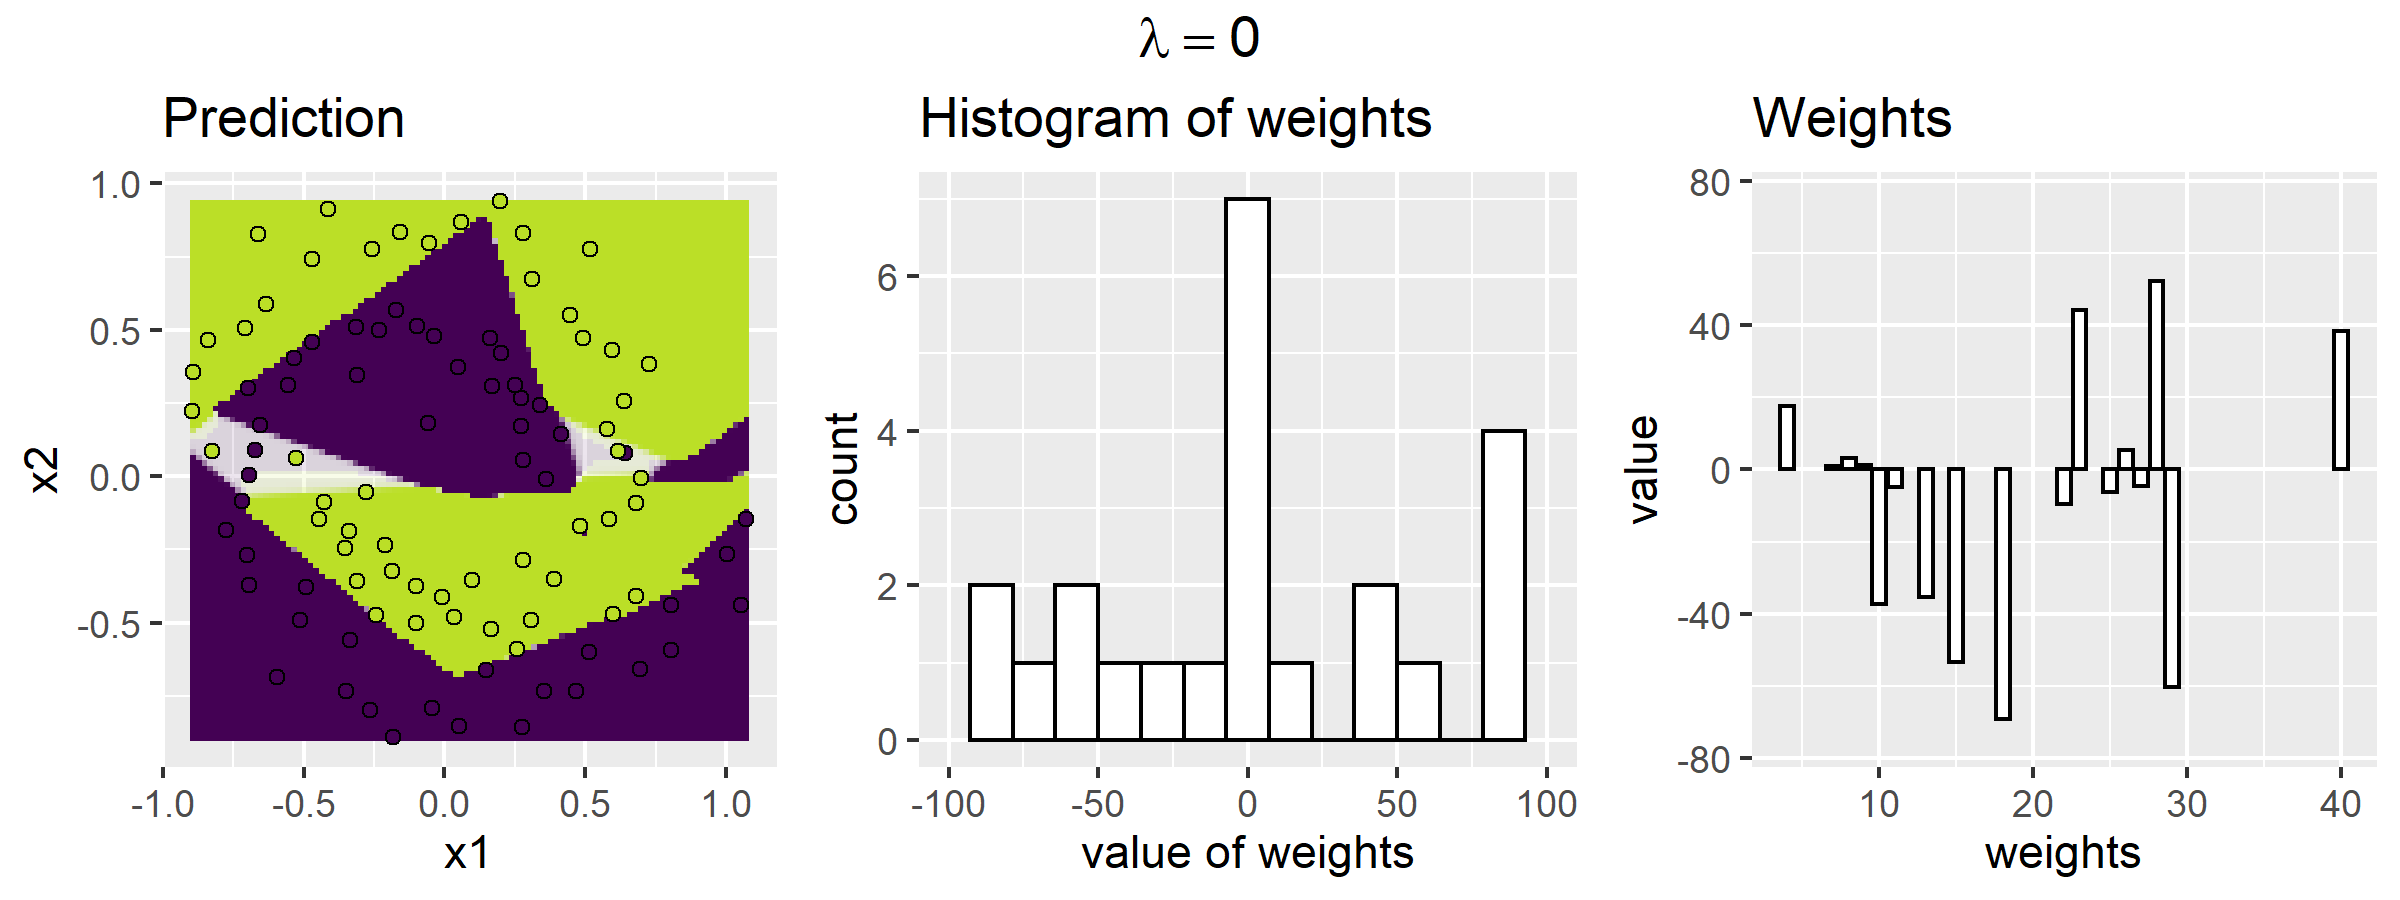
\includegraphics[width=\textwidth]{figure/fig-regu-nonlin-1.png}}
\only<2>{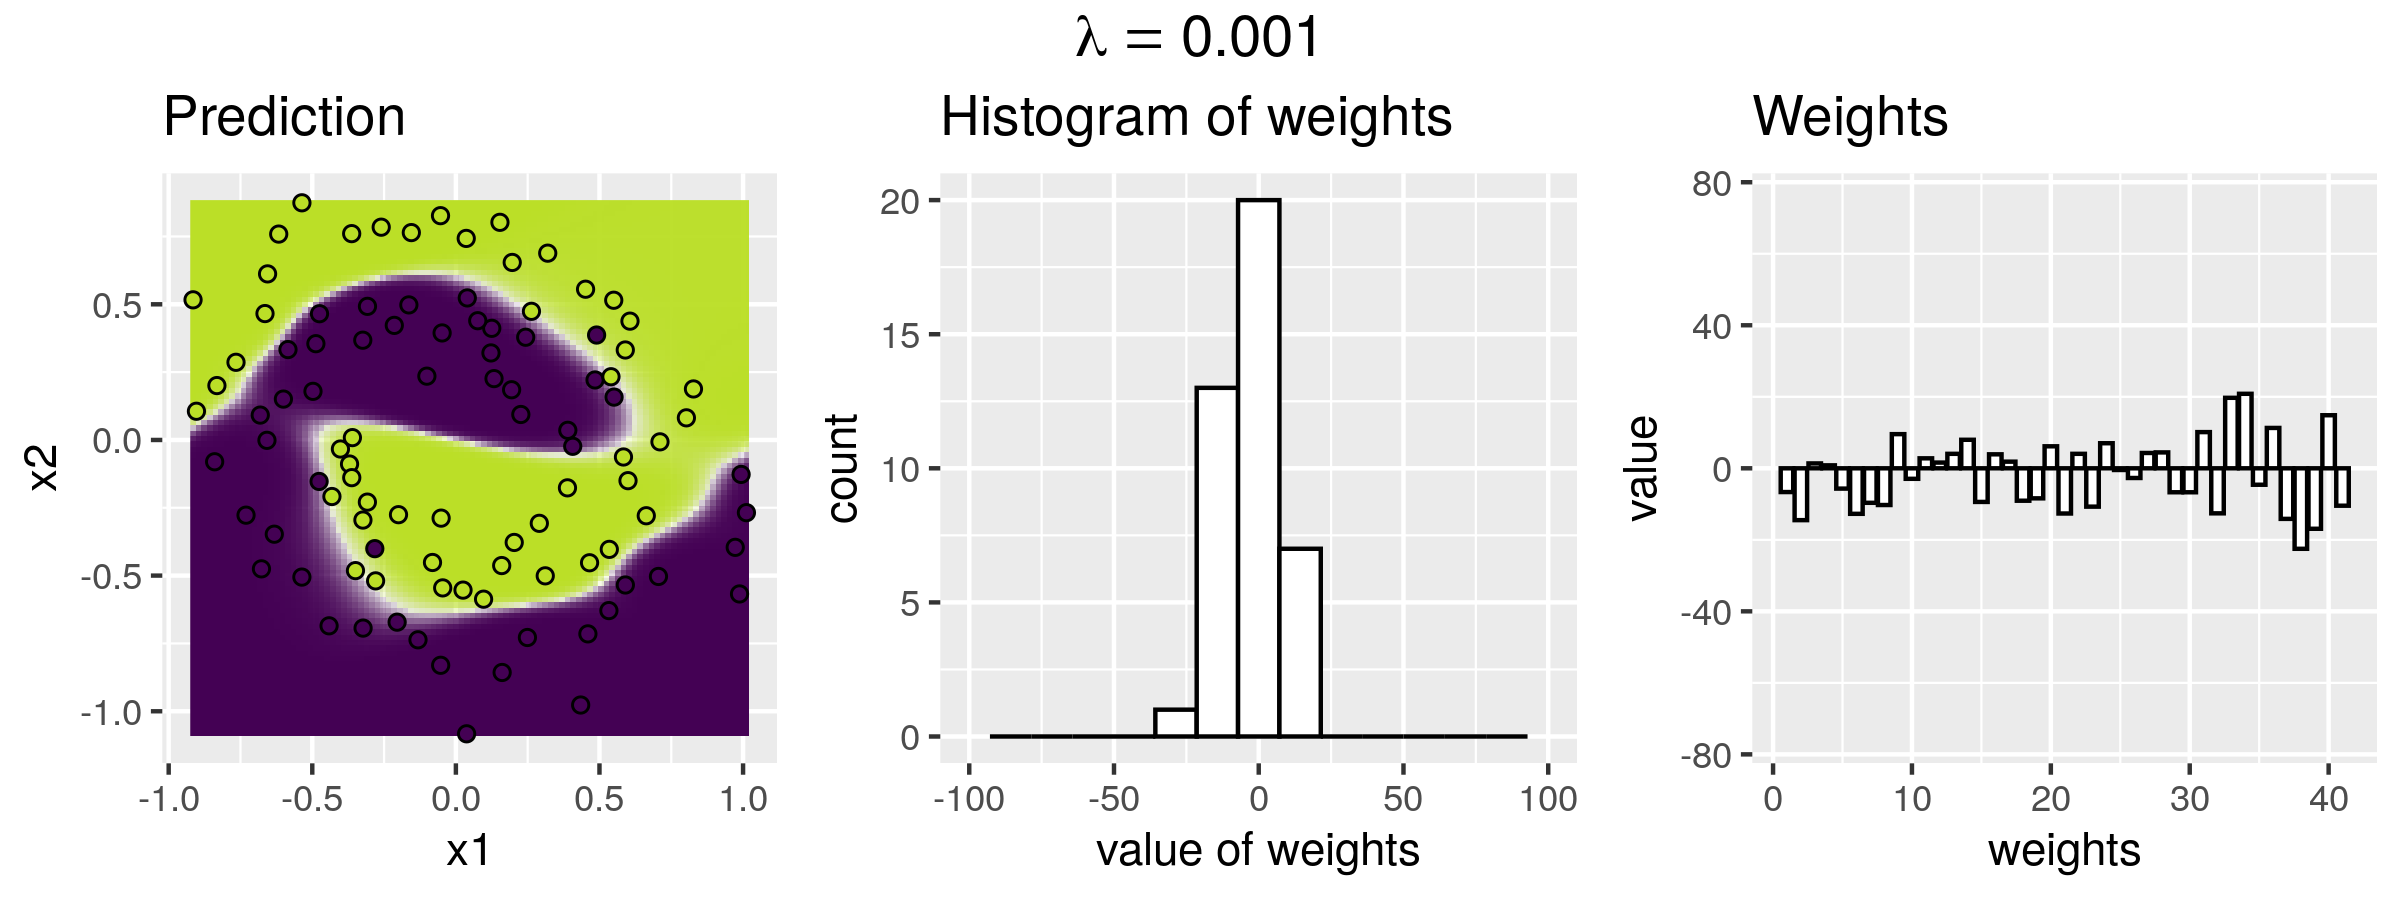
\includegraphics[width=\textwidth]{figure/fig-regu-nonlin-2.png}}
\only<3>{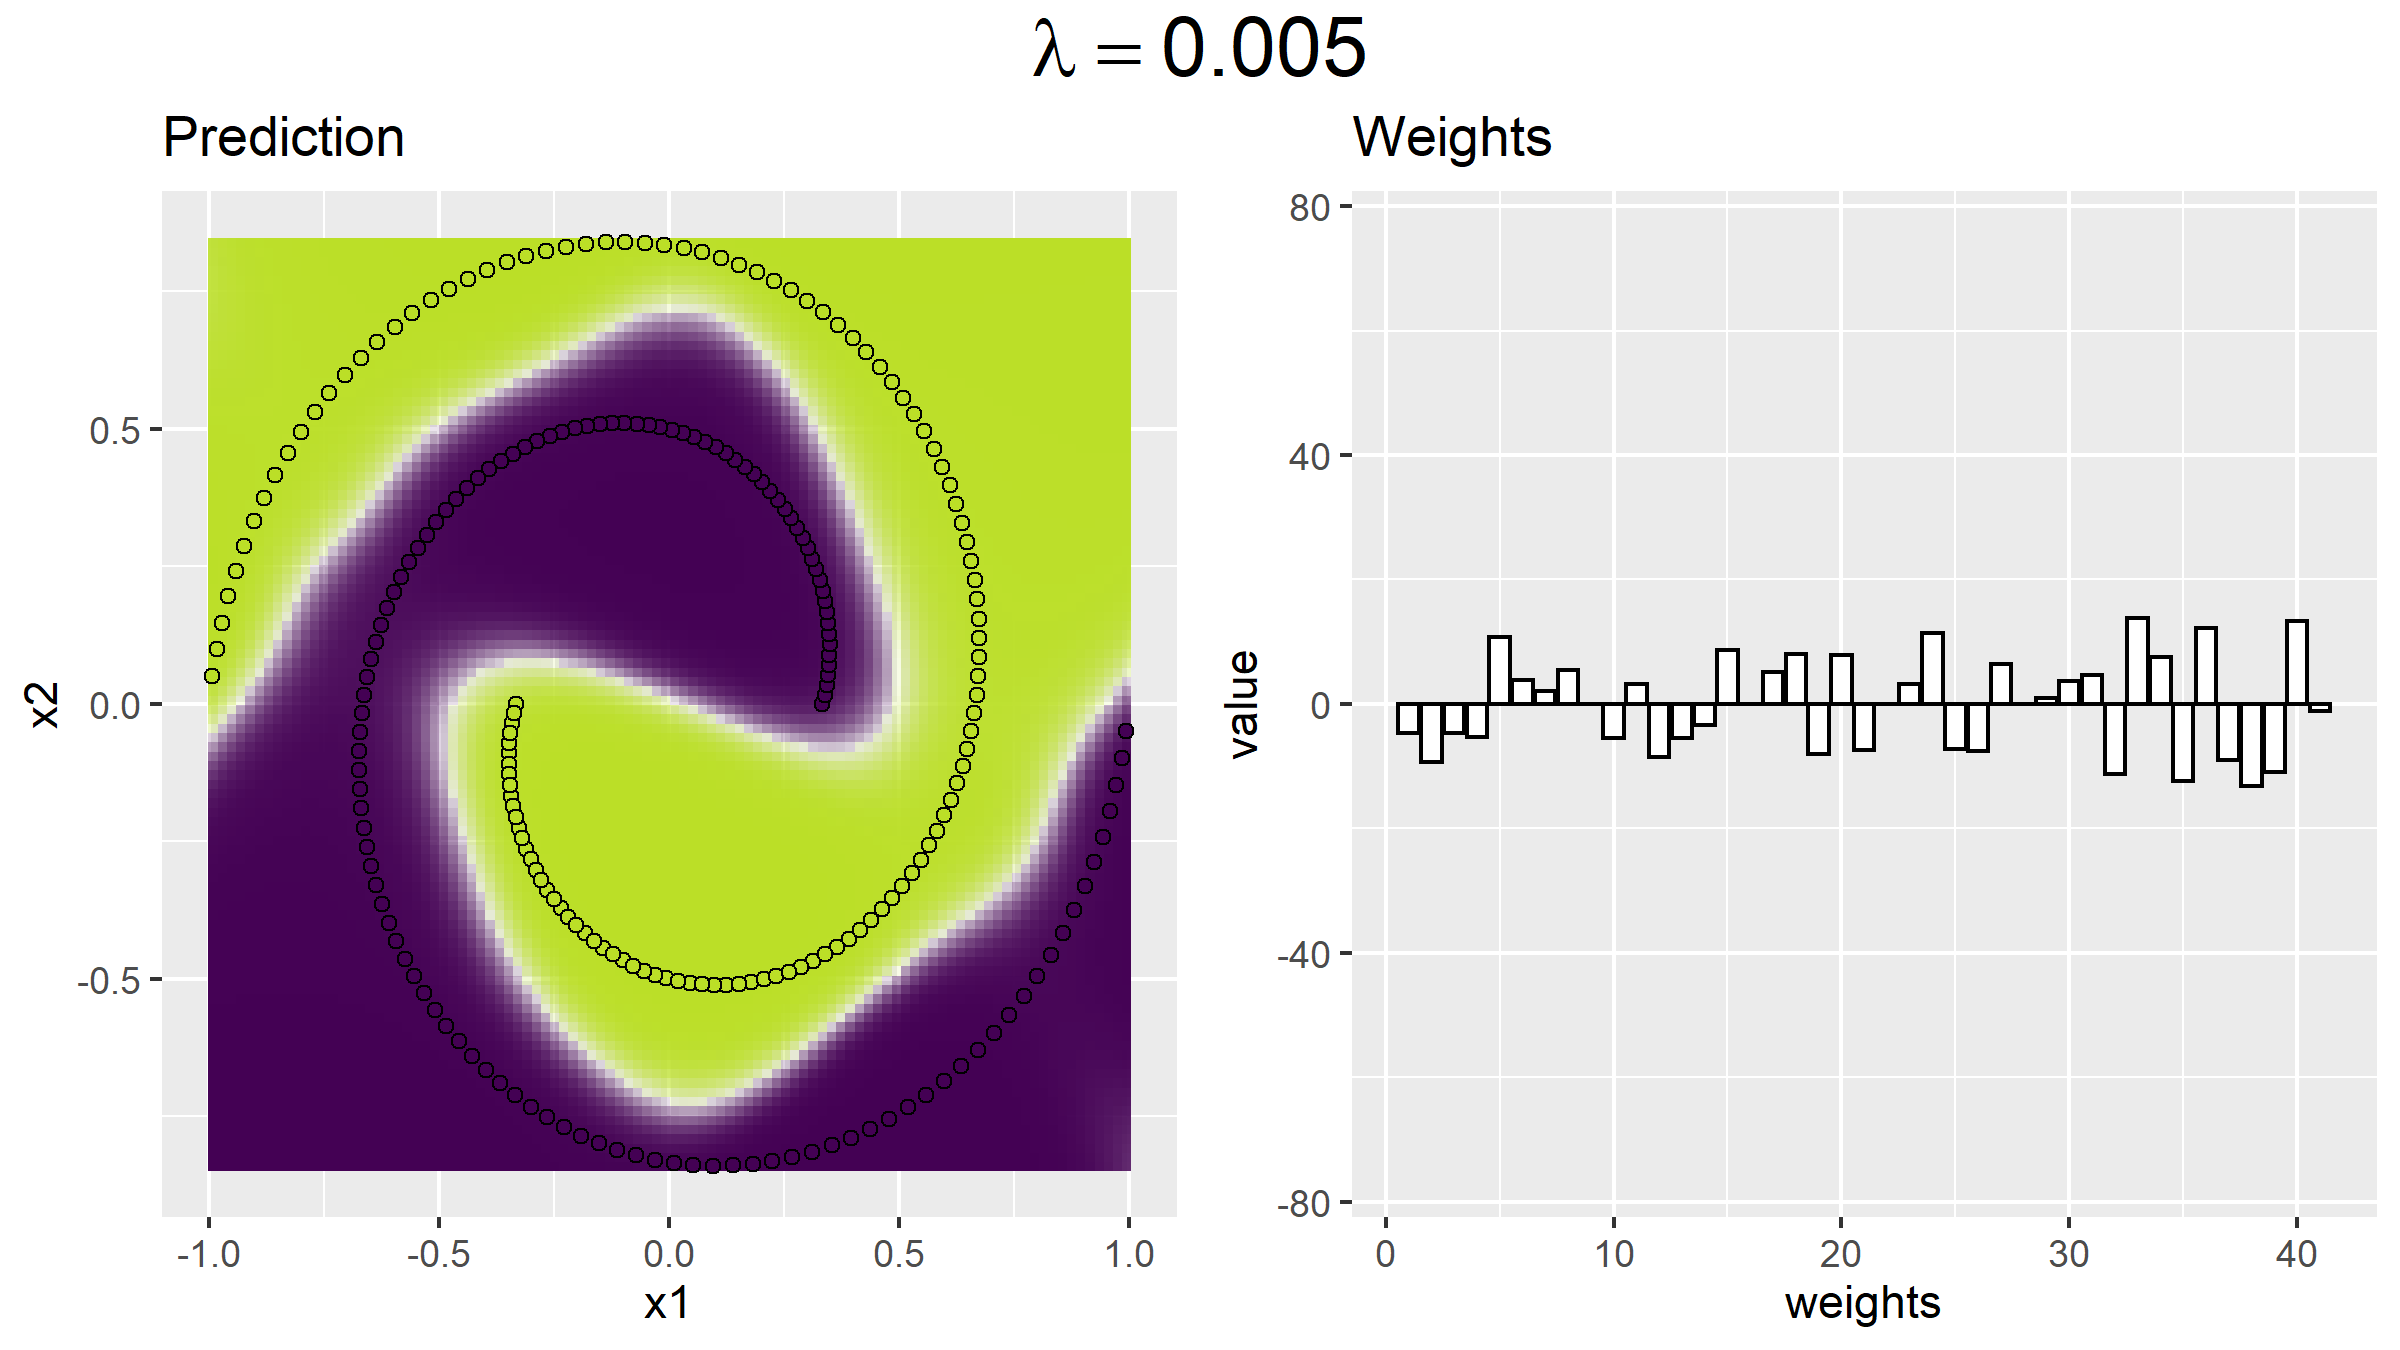
\includegraphics[width=\textwidth]{figure/fig-regu-nonlin-3.png}}
\only<4>{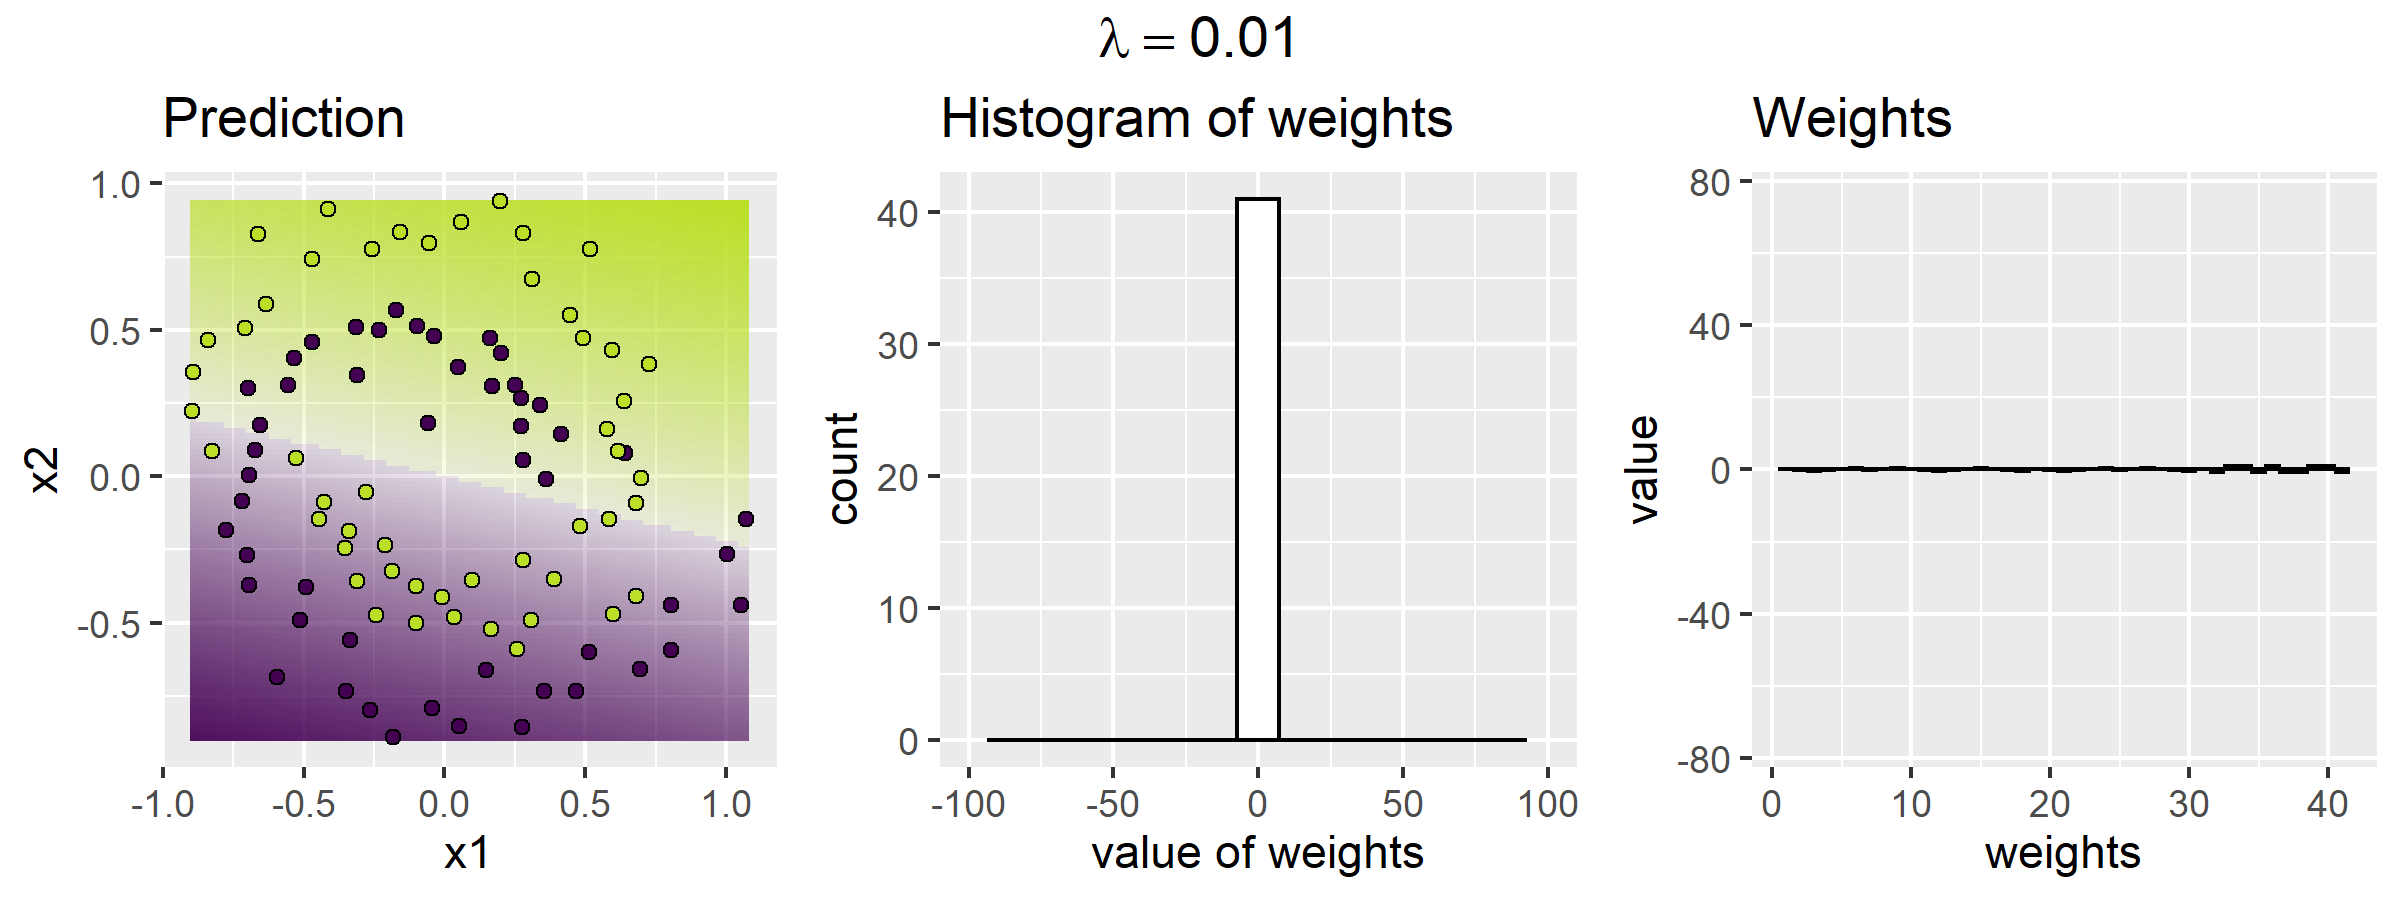
\includegraphics[width=\textwidth]{figure/fig-regu-nonlin-4.png}}
\only<5>{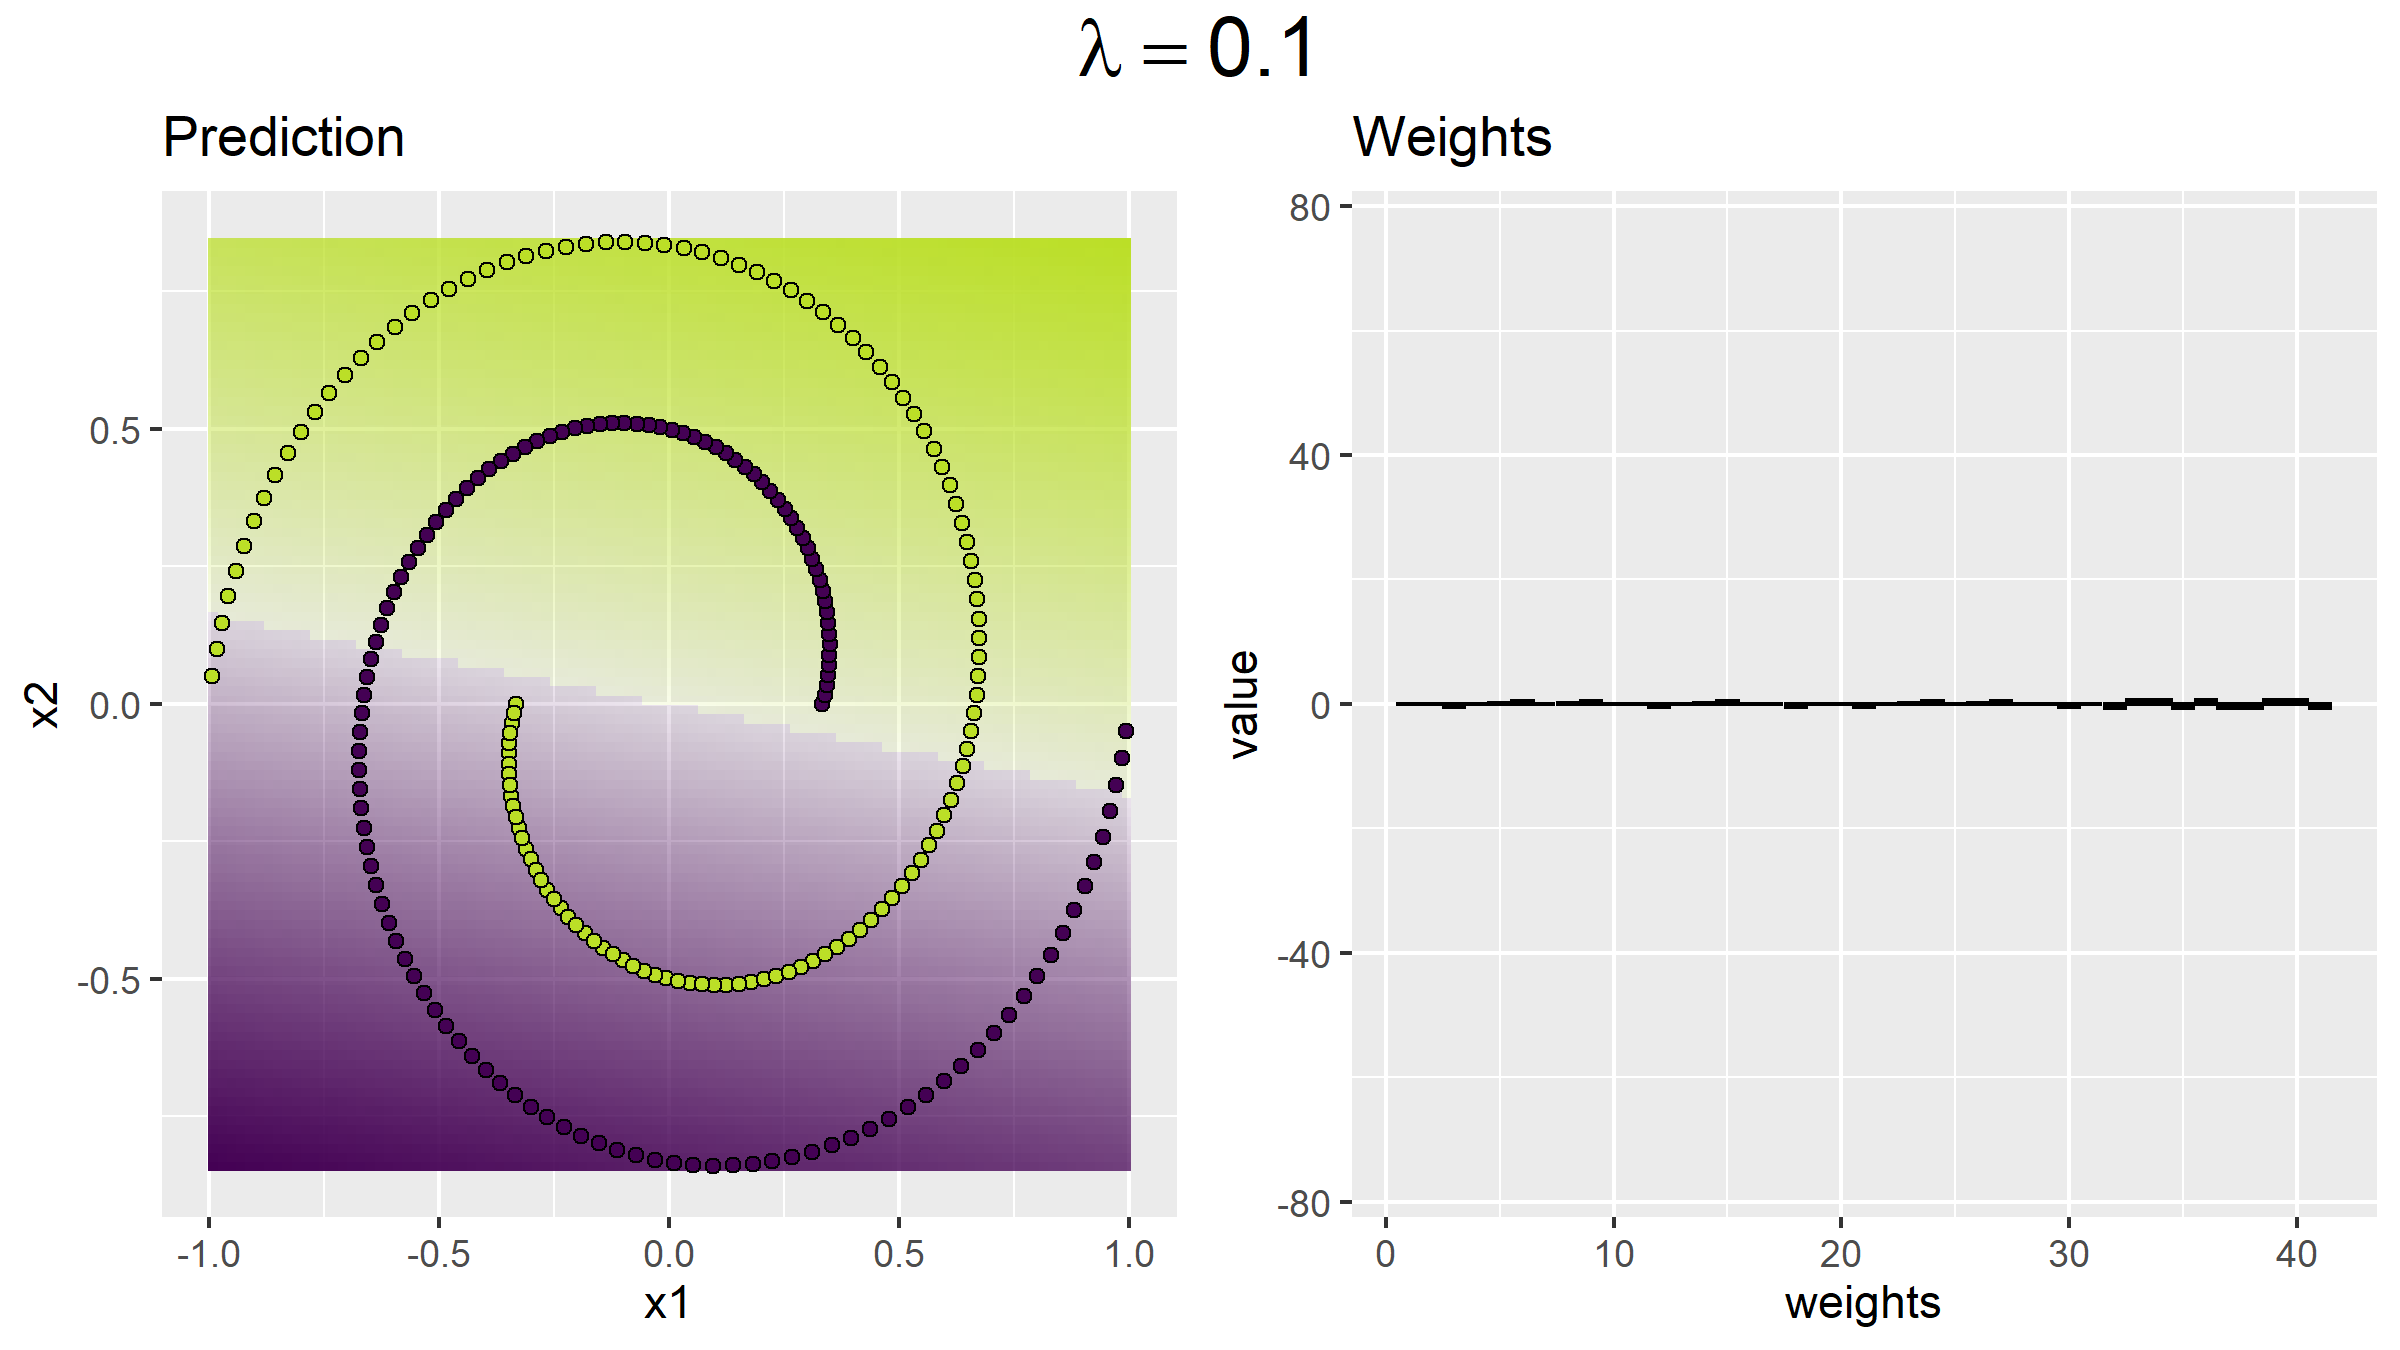
\includegraphics[width=\textwidth]{figure/fig-regu-nonlin-5.png}}
\only<6>{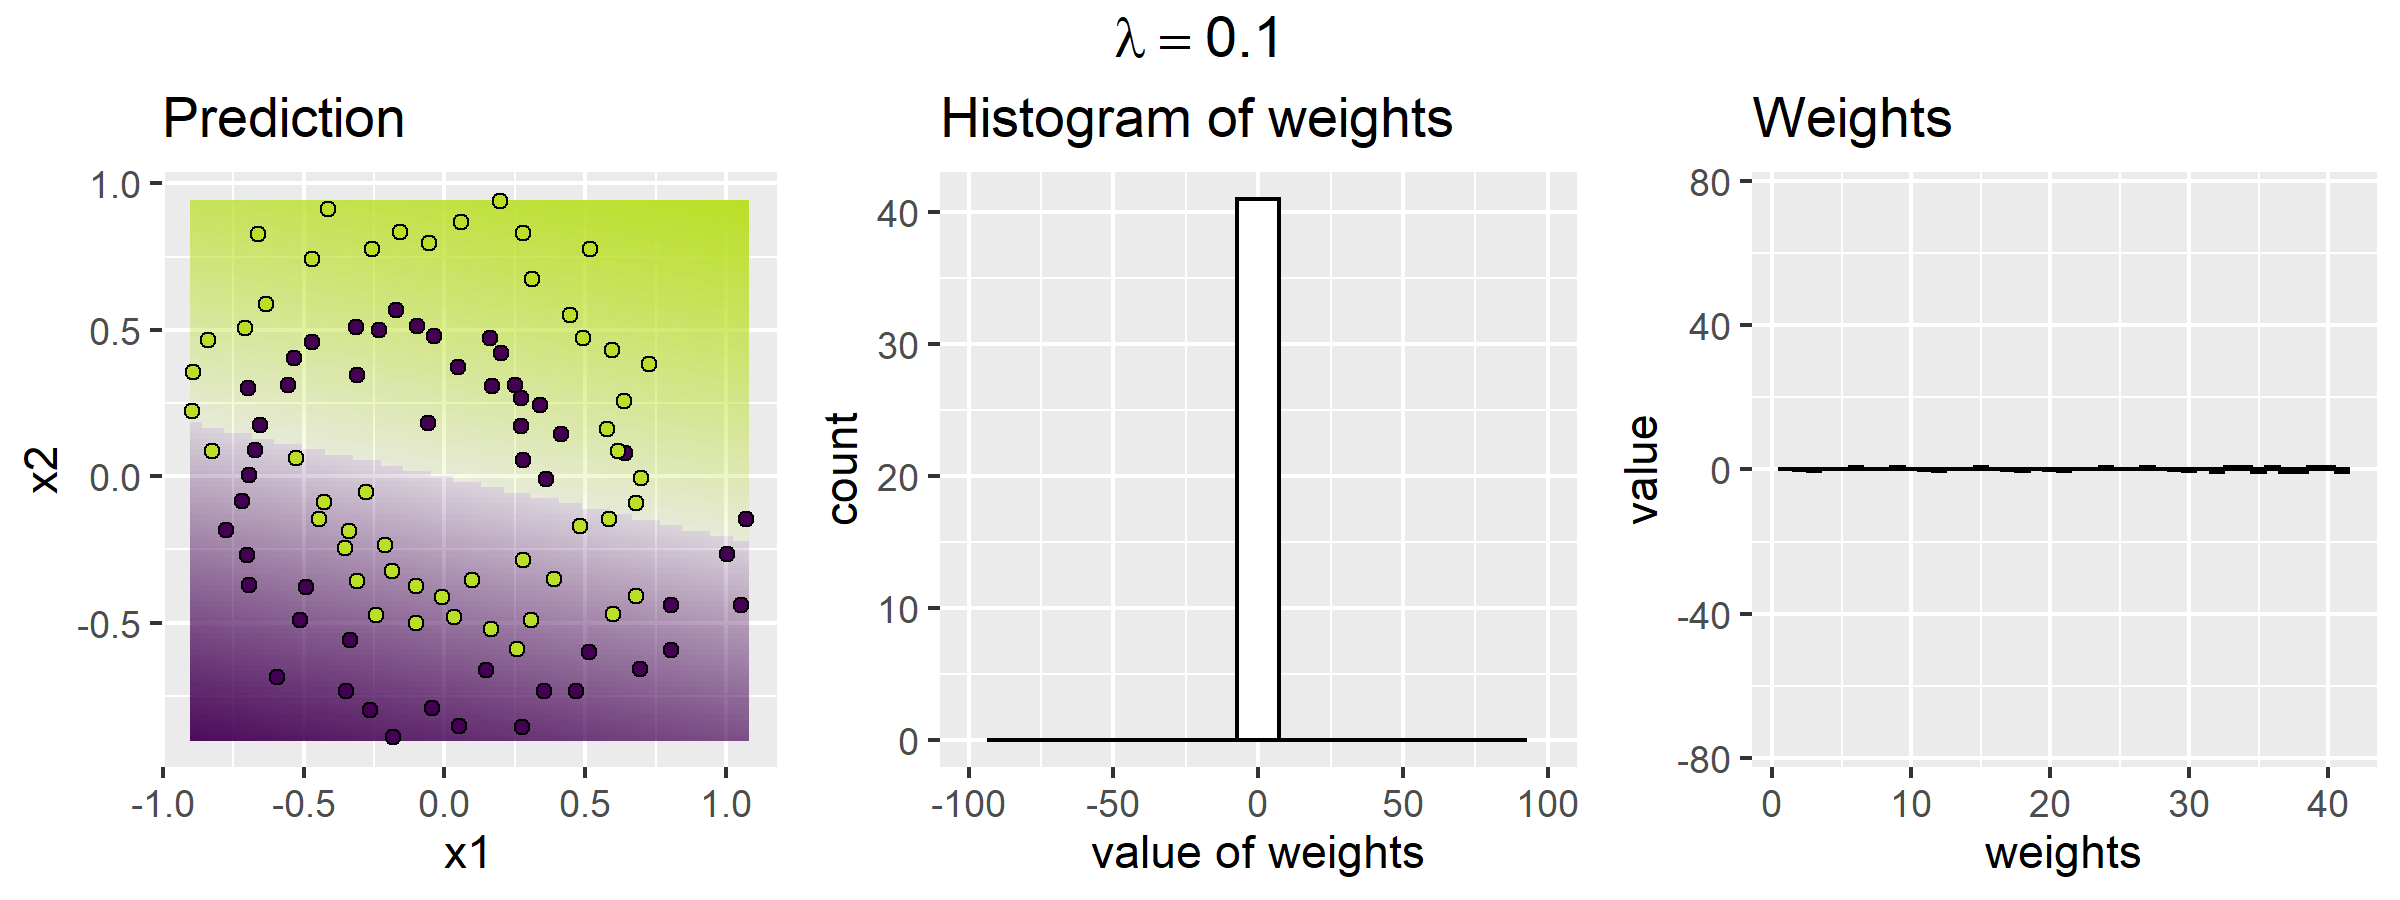
\includegraphics[width=\textwidth]{figure/fig-regu-nonlin-6.png}}
\end{frame}

%-------------------------------------------------------------------------------
\begin{frame}{Non-linear Risk Minimization: Model Complexity}

\small

\textbf{Setting}: Classification for the \texttt{spirals} data.
Neural network with single hidden layer containing 10 neurons and logistic 
output activation and not regularized. 
Varying the size of the hidden layer affects smoothness of the decision boundary:

\vfill

\begin{center}
\only<1>{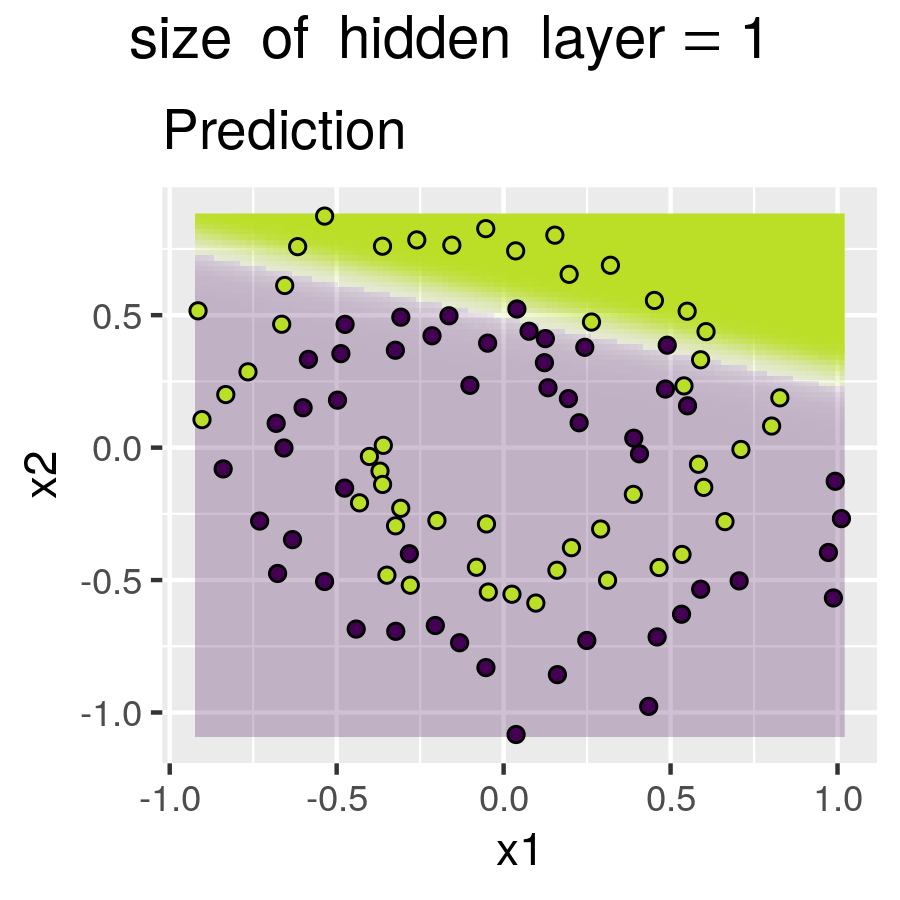
\includegraphics[width=0.5\textwidth]{figure/fig-regu-nonlin-size-1.png}}
\only<2>{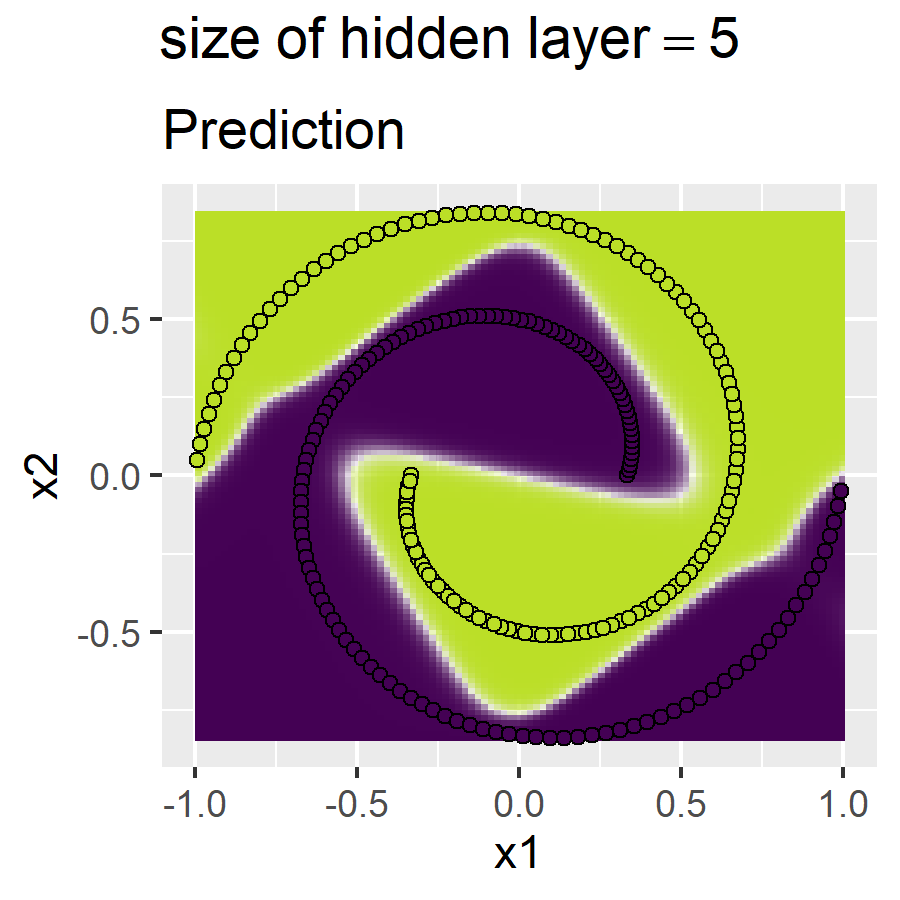
\includegraphics[width=0.5\textwidth]{figure/fig-regu-nonlin-size-2.png}}
\only<3>{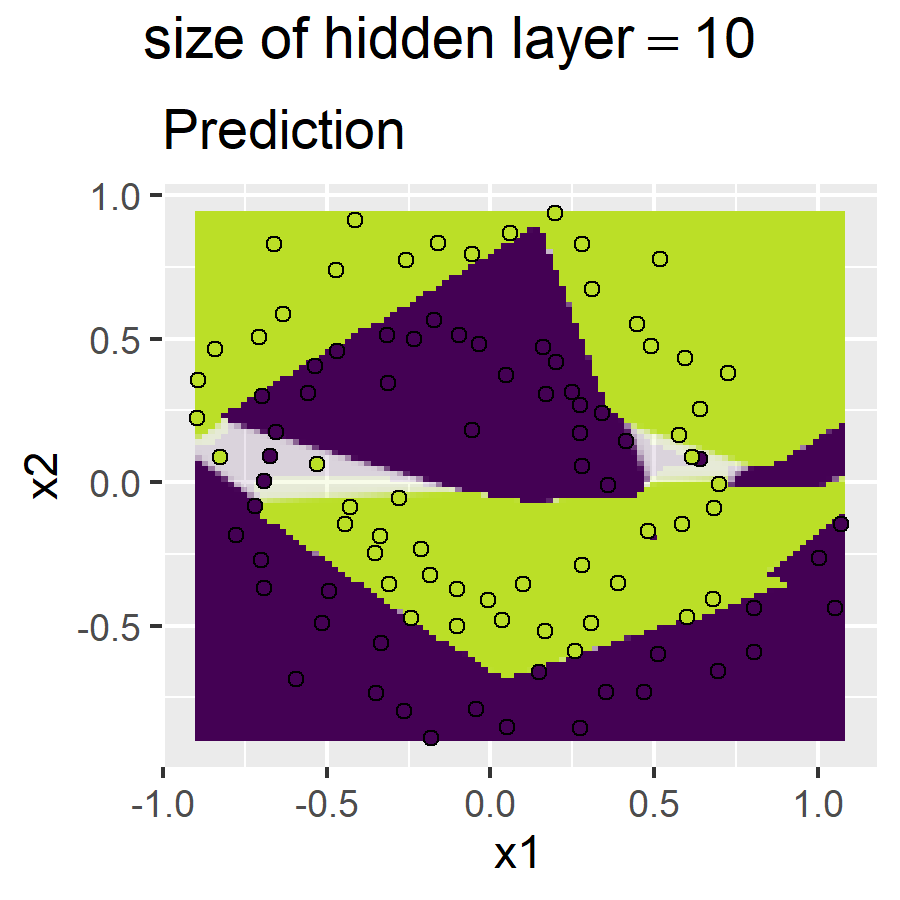
\includegraphics[width=0.5\textwidth]{figure/fig-regu-nonlin-size-3.png}}
\only<4>{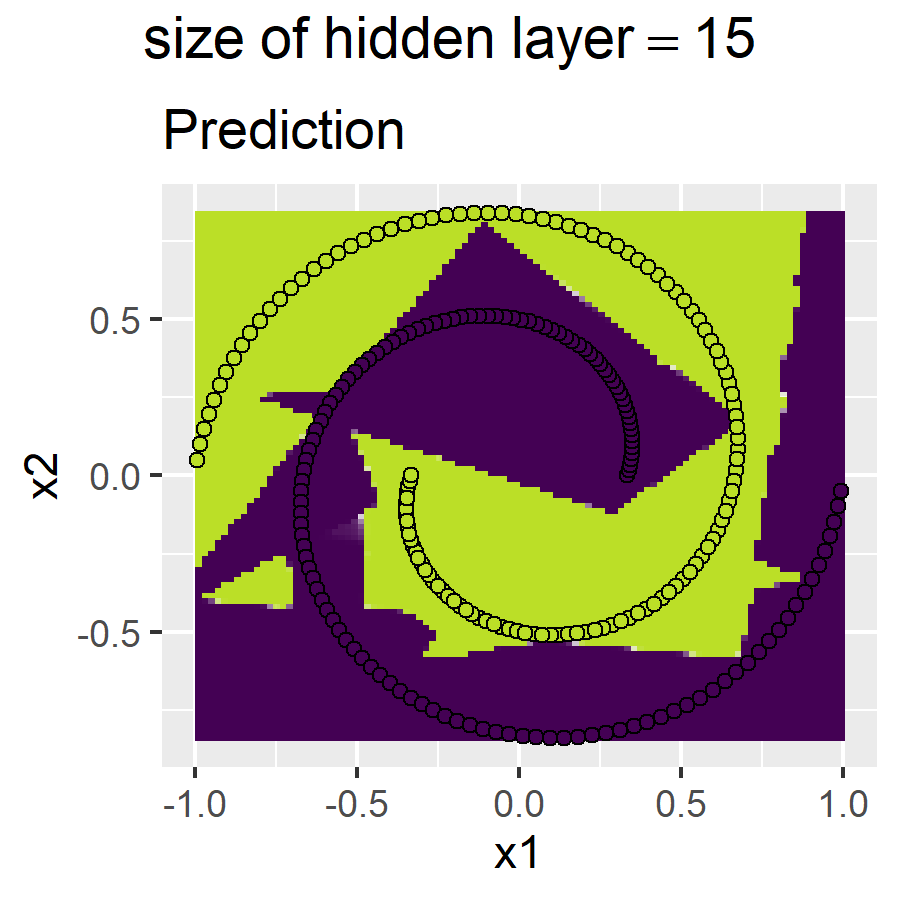
\includegraphics[width=0.5\textwidth]{figure/fig-regu-nonlin-size-4.png}}
\only<5>{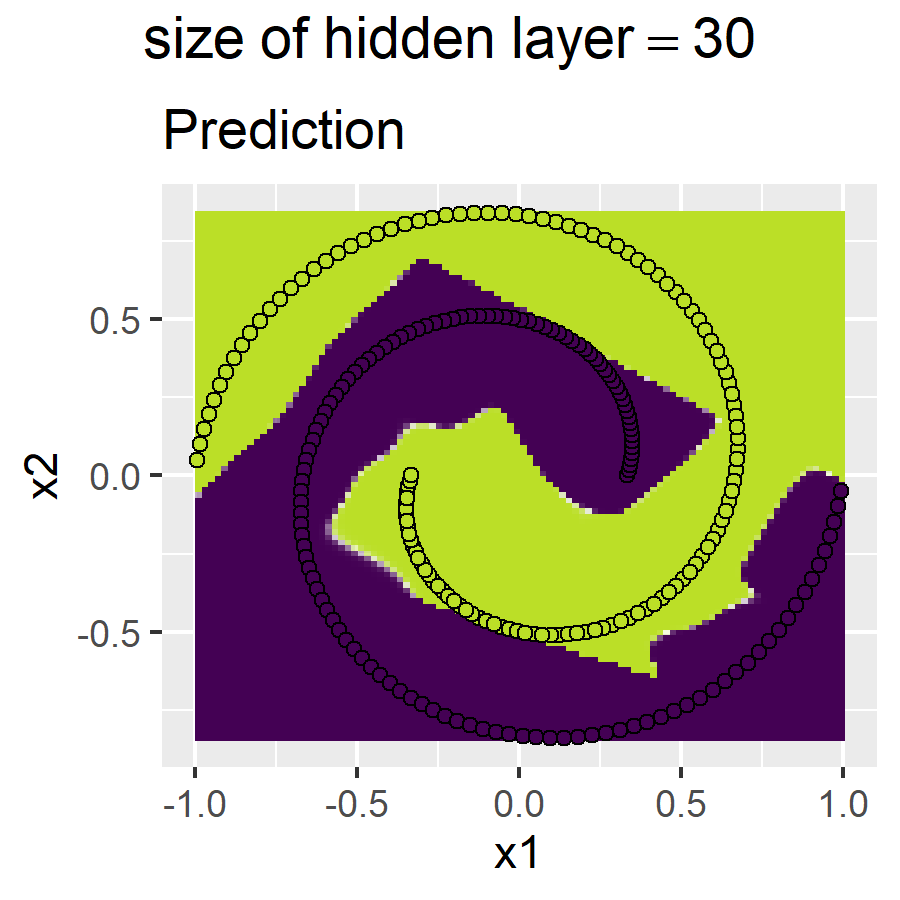
\includegraphics[width=0.5\textwidth]{figure/fig-regu-nonlin-size-5.png}}
\only<6>{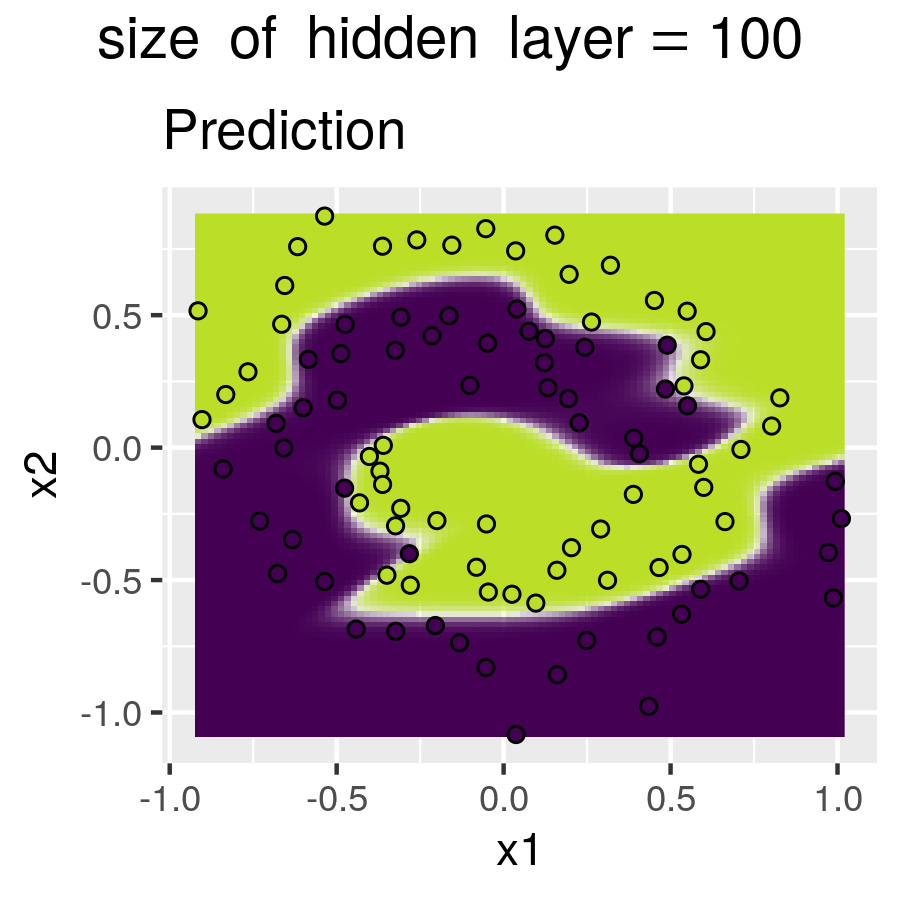
\includegraphics[width=0.5\textwidth]{figure/fig-regu-nonlin-size-6.png}}
\end{center}

\end{frame}

%-------------------------------------------------------------------------------
\begin{vbframe} {Structural Risk Minimization}

\begin{itemize}
  \item Complex models generalize poorly (overfitting) if merely the empirical risk is optimized. 
  \item Thus far, we only considered adding a complexity penalty to empirical risk minimization. 
  \item Instead,  structural risk minimization (SRM) assumes that the hypothesis space $\Hspace$ can be decomposed into increasingly complex hypotheses (size or capacity): $\Hspace = \cup_{k \geq 1 }\Hspace_{k}$. 
  \item Complexity parameters can be the, e.g. the degree of polynomials in linear models or the size of hidden layers in neural networks.  
\end{itemize}

\begin{center}
\includegraphics[width=0.5\textwidth]{figure_man/fig-regu-srm-1}
% FIGURE SOURCE:https://docs.google.com/drawings/d/1qFoFSyuY4glsNvgYgIZ96yRcznOdA5q3oogI5fVBQ1A/edit?usp=sharing
\end{center}

\framebreak


\begin{itemize}

  \item SRM consists of choosing an index $k \geq 1$  and a hypothesis minimizing the empirical risk in $\Hspace_k$, minimizing the generalization error.
  \item By this, the simplest model can be chosen, which minimizes the generalization bound.  
  \item One challenge might be choosing an adequate complexity measure, as for some models, multiple complexity measures exist.
\end{itemize}

\begin{center}
\includegraphics[width=0.7\textwidth]{figure_man/fig-regu-srm-2}
% FIGURE SOURCE: https://docs.google.com/drawings/d/1mk_qVUbfOYwwmuE0AgmnPiNSMoX--pE_nZsWYND0IhQ/edit?usp=sharing
\end{center}

\end{vbframe}
%-------------------------------------------------------------------------------

\section{Regularization from a Bayesian Perspective}

\begin{vbframe} {Regularized Risk Minimization vs. Bayes}

We have already created a link between maximum likelihood estimation and 
empirical risk minimization.

\lz 

Now we will generalize this for regularized risk minimization.

\lz

Assume we have a parameterized distribution $p(\xv | \thetab)$ for our data and 
a prior $q(\thetab)$ over our parameter space, all in the Bayesian framework.

\lz 

With the Bayes theorem we know:

$$
p(\thetab | \xv) = \frac{p(\xv | \thetab) q(\thetab) }{p(\xv)} \propto 
p(\xv | \thetab) q(\thetab)
$$

\framebreak

The maximum a posteriori (MAP) estimator of $\thetab$ is now the minimizer of

$$
- \log p\left(\xv ~|~ \thetab\right) - \log q(\thetab).
$$

\begin{itemize}
  \item Again, we identify the loss $\Lxyt$ with $-\log(p(\xv | \thetab))$.
  \item If $q(\thetab)$ is constant (i.e., we used a uniform, non-informative 
  prior), the second summand becomes irrelevant and we arrive 
  at empirical risk minimization.
  \item If not, we can identify $J(\thetab) \propto -\log(q(\thetab))$, i.e., 
  the log-prior corresponds to the regularizer, and the additional control 
  parameter $\lambda$ corresponds to the relative strength of the prior in 
  regularized risk minimization.
\end{itemize}

\framebreak

\begin{figure}
  \centering
    \scalebox{1}{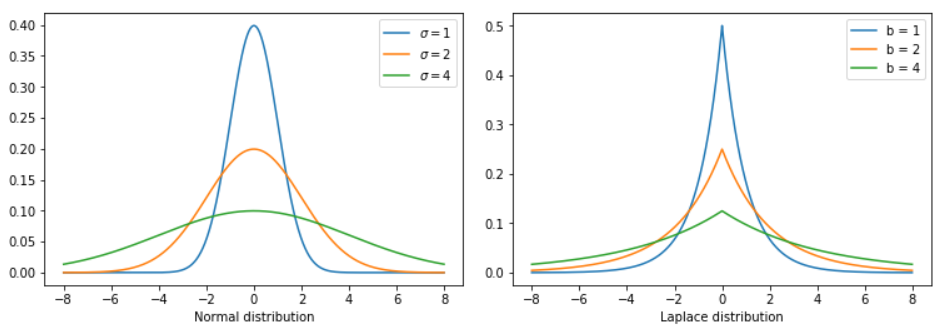
\includegraphics{figure_man/bayes_reg.png}}
\end{figure}

\begin{itemize}
  \item $L2$ regularization corresponds to a zero-mean Gaussian prior with 
  constant variance:
  $\theta_j \sim \mathcal{N}(0, \tau^2) ~ \forall j \in \{1, \dots , d\}$, 
  $\tau > 0$.
  \item The $L1$ analogue for is a zero-mean Laplace prior: 
  $\theta_j \sim \mathit{Laplace}(0,b) = 
  \frac{1}{2b}\exp(-\frac{|\theta_i|}{b})$, where $b$ is a scale parameter.
  \item In both cases, regularization strength $\lambda$ increases as the 
  variance of the prior decreases: a prior probability mass more narrowly 
  concentrated around 0 encourages shrinkage.
\end{itemize}
  
\end{vbframe}

% ------------------------------------------------------------------------------

\begin{vbframe}{Example: Bayesian L2 regularization}

\small We can easily see the equivalence of $L2$ regularization and Gaussian 
priors considering the example of a \textbf{Ridge} penalty term.

\begin{itemize}
  \small
  \item We define a Gaussian prior with uncorrelated components for $\thetab$:
  \begin{footnotesize}
    $$q(\thetab) = \mathcal{N}_d(\bm{0}, \mathit{diag}(\tau^2)) 
    = \prod_{j = 1}^d  \mathcal{N}(0, \tau^2)  
    = (2\pi\tau^2)^{-\frac{d}{2}} \exp \left( \frac{1}{2\tau^2} \sum_{j = 1}^d 
    \theta_j^2 \right).$$
  \end{footnotesize} 
  \item With this, the MAP estimator becomes
  \begin{footnotesize}
  \begin{eqnarray*}
    \thetah^{\text{MAP}} &=& argmin_{\thetab} \left(
    - \log p\left(\xv ~|~ \thetab\right) - \log q(\thetab)
    \right) \\
    &=& \argmin_{\thetab} \left(
    - \log p\left(\xv ~|~ \thetab\right) + \tfrac{d}{2} \log(2\pi \tau^2) +
    \frac{1}{2\tau^2} \sum_{j = 1}^d \theta_j^2
    \right) \\
    &=& \argmin_{\thetab} \left(
    - \log p\left(\xv ~|~ \thetab\right) + \frac{1}{2\tau^2} {\thetab}^T\thetab 
    \right) \\
    &=& \argmin_{\thetab} \left(
    - \log p\left(\xv ~|~ \thetab\right) + \frac{1}{2\tau^2} \| \thetab \|_2^2
    \right).
  \end{eqnarray*}
  \end{footnotesize} 
  % \item $\frac{1}{\tau^2}$ controls prior precision, i.e., inverse variance, 
  % and thus the amount of shrinkage.
  \item We see how the inverse variance $\tau^2$ controls shrinkage.
  % (e.g., for linear Ridge regression with 
  % $\epsilon \sim \mathcal{N}(0, \sigma^2)$ we set 
  % $\lambda = \frac{\sigma^2}{\tau^2}$).
\end{itemize}
  
  % \item The conditional distribution of $\ydat$ in linear regression with 
  % Gaussian errors $\epsilon^{(i)} \sim \mathcal{N}(0, \sigma^2) ~ \forall i \in 
  % \setn$, $\sigma > 0$, is also Gaussian: 
  % \begin{footnotesize}
  % $$- \log p\left(\ydat ~|~ \xv, \thetab\right) = \frac{n}{2} \log (2\pi 
  % \sigma^2) + \frac{1}{2\sigma^2} \sumin \left(\yi - \fxit \right)^2.$$
  % \end{footnotesize}

% &=& \argmin_{\thetab} \left(
% \tfrac{n}{2} \log (2\pi \sigma^2) + \frac{1}{2\sigma^2} \sumin \left(\yi -
% \fxit \right)^2 + \tfrac{p}{2} \log(2\pi \tau^2) +
% \frac{1}{2\tau^2} \sumjp \theta_j^2
% \right) \\
% &=& \argmin_{\thetab} \left( \frac{1}{\sigma^2} \sumin \left(\yi -
% \fxit \right)^2 + \frac{1}{\tau^2} \sumjp \theta_j^2 \right) \\
% &=& \argmin_{\thetab} \left(
% \frac{1}{\sigma^2} \left(\ydat - \Xmat \thetab\right)^\top \left(\ydat - \Xmat
% \thetab\right) + \frac{1}{\tau^2} {\thetab}^T\thetab
% \right)

% \begin{eqnarray*}
% \thetah^{\text{MAP}} &=& argmin_{\thetab} \left(
% - \log p\left(\ydat ~|~ \xv, \thetab\right) - \log q(\thetab)
% \right) \\
% 
% &=& \argmin_{\thetab} \left(
% \tfrac{n}{2} \log (2\pi \sigma^2) + \frac{1}{2\sigma^2} \sumin \left(\yi -
% \fxit \right)^2 + \tfrac{p}{2} \log(2\pi \tau^2) +
% \frac{1}{2\tau^2} \sumjp \theta_j^2
% \right) \\
% &=& \argmin_{\thetab} \left( \frac{1}{\sigma^2} \sumin \left(\yi -
% \fxit \right)^2 + \frac{1}{\tau^2} \sumjp \theta_j^2 \right) \\
% &=& \argmin_{\thetab} \left(
% \frac{1}{\sigma^2} \left(\ydat - \Xmat \thetab\right)^\top \left(\ydat - \Xmat
% \thetab\right) + \frac{1}{\tau^2} {\thetab}^T\thetab
% \right)
% 
% &=& \argmin_{\thetab} \left(
% \tfrac{n}{2} \log (2\pi \sigma^2) + \frac{1}{2\sigma^2} \sumin \left(\yi -
% \fxit \right)^2 + \tfrac{p}{2} \log(2\pi \tau^2) +
% \frac{1}{2\tau^2} \sumjp \theta_j^2
% \right) \\
% &=& \argmin_{\thetab} \left( \frac{1}{\sigma^2} \sumin \left(\yi -
% \fxit \right)^2 + \frac{1}{\tau^2} \sumjp \theta_j^2 \right) \\
% &=& \argmin_{\thetab} \left(
% \frac{1}{\sigma^2} \left(\ydat - \Xmat \thetab\right)^\top \left(\ydat - \Xmat
% \thetab\right) + \frac{1}{\tau^2} {\thetab}^T\thetab
% \right)
% \end{eqnarray*}

% \footnotesize
% Now, define $\lambda := \frac{\sigma^2}{\tau^2}$ -- note how higher prior 
% precision (i.e., lower variance) increases shrinkage! -- and set the derivative 
% to 0:
% 
% \begin{scriptsize}
% \begin{eqnarray*}
% 0 &=& \frac{1}{\lambda \tau^2} \left( - {\Xmat}^T \ydat + \thetab {\Xmat}^T \Xmat
% \right) + \frac{\lambda}{\sigma^2} \thetab
% \quad \Leftrightarrow \quad 0 = \frac{\sigma^2}{\tau^2} \left( - {\Xmat}^T \ydat 
% + \thetab {\Xmat}^T \Xmat \right) + \lambda^2 \thetab \\
% 0 &=&  - {\Xmat}^T \ydat + \thetab {\Xmat}^T \Xmat + \lambda \thetab 
% \quad \Leftrightarrow \quad 
% \thetab(\Xmat^T \Xmat  + \lambda \id) = {\Xmat}^T \ydat
% \end{eqnarray*}
% \end{scriptsize}
% 
% $\Rightarrow \thetah^{\text{MAP}} = 
% (\Xmat^T \Xmat  + \lambda \id)^{-1} \Xmat^T\ydat  = \thetah^{\text{Ridge}}.$

\end{vbframe}

% ------------------------------------------------------------------------------

% \begin{vbframe} {Minimum Description Length}

% MDL principle

% \begin{itemize}
%   \item (Compress data using using fewer symbols than literal)
%   \item (In the MDL framework, learning is seen as data compression)
%   \item (More we compress, more we learn. Therefore, pick the hypothesis which results in the shortest code.)
%   \item (Occam's razor, principle of parsimony)
%   \item (All else being equal, a simpler explanation is better than a complex one.)
% \end{itemize}

% % \begin{equation}
% %     \begin{aligned}
% %     H_{\mathrm{mdl}} & :=\underset{H \in \mathcal{H}}{\arg \min }\left(L(H)+L_{H}(D)\right) \\
% %     L_{\mathrm{mdl}}(D) & :=\min _{H \in \mathcal{H}}\left(L(H)+L_{H}(D)\right)
% %   \end{aligned}
% % \end{equation}

% \framebreak

% \begin{itemize}
%   \item There is a correspondence between the length of a message L(x) and the distribution P(x)
%   $$P(x)=2^{-L(x)}, \quad L(x)=-\log _{2} P(x)$$
%   \item Two-part code : parameter block and data block
%   \item $L(H)$ is the length of a specific hypothesis in the set.
%   \item $L(D|H)$ is the length of the data encoded under H.
%   \item $L(D,H) = L(H) + L(D|H)$
%   \item (Represents a tradeoff between goodness-of-fit and complexity)
% \end{itemize}

% \framebreak

% Regression example : $Y_{i}=f\left(X_{i}\right)+\epsilon_{i} \text { for } i=1, \ldots, n \text { where } \epsilon_{i} \stackrel{i i d}{\sim} \mathcal{N}\left(0, \sigma^{2}\right)$

% For a given dataset, the length of the encoding is :

% $$\log 1 / p_{Y | X}\left(y^{n} | x^{n}\right) = \log \left(\sqrt{2 \pi \sigma^{2}} e^{\frac{1}{2 \sigma^{2}} \sum_{i=1}^{n}\left(y_{i}-f\left(x_{i}\right)\right)^{2}}\right) \propto \sum_{i=1}^{n}\left(y_{i}-f\left(x_{i}\right)\right)^{2}$$

% \lz

% The two-stage MDL procedure to pick the best hypothesis is :

% $$f_{\gamma}=\arg \min _{f \in F_{\gamma}}\left[L(f)+\frac{1}{n} \sum_{i=1}^{n}\left(Y_{i}-f\left(X_{i}\right)\right)^{2}\right]$$

% This is equivalent to regularized least squares.
% \end{vbframe}




%%%%%%%%%%%%%%%%%%%%%%%%%%%%%%%%%%%%%%%%%%%%%%%%%%%%%%%%%%%%%%%%%%
%%%%%%%%%%%%%%%%%%          REFERENCES          %%%%%%%%%%%%%%%%%%
%%%%%%%%%%%%%%%%%%%%%%%%%%%%%%%%%%%%%%%%%%%%%%%%%%%%%%%%%%%%%%%%%%
% \begin{vbframe}
% \frametitle{References}
% \footnotesize{
% \begin{thebibliography}{99}

% %%%%%%%%%%%%%%%%%%%%%%%%%%%%%%%%%%
% \bibitem[Ian Goodfellow et al., 2016]{5} Ian Goodfellow, Yoshua Bengio and Aaron Courville (2016)
% \newblock Deep Learning
% \newblock \emph{\url{http://www.deeplearningbook.org/}}

% \end{thebibliography}
% }
% \end{vbframe}


\endlecture
\end{document}

